%!TEX root = ../Thesis.tex

\chapter{Experimentos y resultados}\label{ch:chap6}

\epigraphhead[70]{
\epigraph{``Data! Data! Data!'' he cried impatiently. 
``I can't make bricks without clay.''}{Sherlock Holmes}}

En los capítulos anteriores se ha descrito los diferentes algoritmos que se utilizarán para realizar la tarea de \sd, y que en esta sección se emplearán de acuerdo al marco experimental que se describe a continuación.

Inicialmente, las pruebas consistieron en usar los algoritmos presentados para selección de modelo usando datos que fueron generados aleatoriamente a partir de los parámetros de un \ac{HMM} inicial; para tener una idea general de su desempeño individual.

Para estas primeras pruebas, se simuló una cadena de Márkov oculta con base en parámetros fijos, generando tanto una secuencia de datos observados, como los supuestos datos o variables ocultas que forman la cadena de Márkov. Se utilizó muestreo ancestral para la simulación de estos datos.

Para un caso en específico, se tiene lo siguiente. Realizando la inferencia de parámetros del \ac{HMM}, se obtienen los siguientes resultados:

El primer algoritmo que se prueba, es el de selección de modelo usando un \ac{BIC}.

Como ya se comentó, se usará una variante de \ac{BIC} en donde se incorpora un término de regularización $\lambda$ para que correspondan en órdenes de magnitud tanto la log-verosimilitud del modelo encontrado como su penalización respectiva.

El problema inmediato que se presenta, es cómo realizar la selección del parámetro de regularización $\lambda$ que penalice de forma correcta la verosimilitud para los diferentes modelos propuestos. Si $\lambda$ es demasiado pequeño, entonces la penalización realmente no tendrá efecto y dado el sobre ajuste que se presenta al usar modelos más complejos, se preferirán siempre los modelos con más parámetros. Por otro lado, si al escoger $\lambda$ se da demasiado peso al término de regularización, entonces siempre se preferirán los modelos más sencillos.

Para encontrar el valor de $\lambda$ adecuado, se puede entonces formar una superficie con las diferentes curvas de selección \ac{BIC} de acuerdo a cómo varía $\lambda$, e inspeccionar esta superficie para encontrar una región de confianza en la que el valor de $\lambda$ es el adecuado.

Por otro lado, para la segunda prueba, se procedió a usar bootstrap con la estadística \ac{LLR} como ya se describió anteriormente en el \autoref{ch:chap3}, y haciendo la prueba de hipótesis del modelo de $n$ estados contra el de $n+1$ estados.

\section{Experimentos} % (fold)
\label{sec:experimentos}

Para los experimentos realizados, se generaron mediante un \ac{TTS} para la generación de las secuencias de prueba, lo que nos permitió tener un mayor control sobre el contenido como tal de las grabaciones, así como sobre los posibles ruidos o interferencias en la señal de audio.

Si bien, para probar el desempeño contra otras propuestas del estado del arte se suelen usar otro tipo de bases de datos (tales como \ac{NIST}, ...), éstas suelen no estar disponibles de forma libre, por lo que preferimos generar nosotros un conjunto de pruebas con el sintetizador de voz.

Usando dos motores para el sintetizador de voz, uno con voces en inglés y otro con voces en español, se generaron 6 secuencias de audio (3 en cada idioma) cuya duración así como el número de interlocutores que participan varía.

\subsection[Secuencia 1]{Secuencia 1: Edgar Allan Poe} % (fold)
\label{ssub:allanpoe}

  En esta primer secuencia se tomaron varios poemas del escritor Edgar Allan Poe, y se utilizaron 6 diferentes voces en inglés. La secuencia de audio original es de 12:06 min.

Para la etapa de agrupación de los vectores MFCC con k-means++ se usaron 140 centros iniciales, mientras que el banco de filtros fue el mismo que anteriormente se mencionó.

\begin{figure}[tp]
  \centerline{  
    \hspace{1.2cm}
    \parbox[c]{0.38\textwidth}{\centering Modelo generador}
    \parbox[c]{0.38\textwidth}{\centering Modelo $n_4$}
    \parbox[c]{0.38\textwidth}{\centering Modelo $n_5$}
    \parbox[c]{0.38\textwidth}{\centering Modelo $n_6$}
  }
  \vspace{0.5cm}
  \foreach \row in {1, ..., 2}{%  
    \centerline{%
      \parbox[c]{1cm}{
        \vspace{-0.5cm}
        \myheader{\row}
      }
      %\gdef \widthimg {0.35}
      \foreach \col in {1, ..., 4}{%
        \pgfmathparse{\col == 4 && \row == 2? 1:0}
        \ifthenelse{\pgfmathresult=1}{
          \gdef \widthimg {0.39}
        }{
          \gdef \widthimg {0.35}
        }
        \begin{subfigure}[c]{\widthimg \textwidth}          
          \def \imgfile {gfx/chap6/cuervo1p_\col_\row}
          \IfFileExists{\imgfile.eps}{
            \includegraphics[width=1\textwidth]{\imgfile}
            \label{fig:seq1p_\col_\row}
          }{
            \hspace{1\textwidth}
          }
        \end{subfigure}
        %\hspace{-0.005\textwidth}
      }
    }
  }
\caption[Secuencia 1: Parámetros estimados (1)]{Por columnas, se muestran los parámetros obtenidos para varios modelos propuestos. La primer columna corresponde a los parámetros verdaderos.
En la primer fila \textup{(a)} se muestran las probabilidades a priori de que cada uno de los interlocutores empiecen la conversación. En la segunda fila \textup{(b)} se muestra en falso color la matriz de transición entre interlocutores para cada uno de los modelos mostrados.}
\label{fig:seq1p}
\end{figure}

En las \autoref{fig:seq1p} y \autoref{fig:seq1q} se muestran los parámetros estimados para los diferentes modelos que se propusieron. La primer columna corresponde a los parámetros verdaderos, mientras que las demás columnas son los parámetros obtenidos para diferentes modelos estimados. 

En la primer fila de la \autoref{fig:seq1p} se muestran las probabilidades a priori de que cada uno de los interlocutores empiecen el diálogo. En la segunda fila se muestra en falso color la matriz de transición para cada uno de los modelos. Esta matriz representa la probabilidad de cambio entre las personas que participan en la conversación.

Se observa como en general para todos los modelos propuestos la matriz de transición que se recupera tiene una estructura diagonal, puesto que en este tipo de problemas, una persona suele hablar durante un periodo considerablemente largo, para que luego otra persona empiece a hablar.

\begin{figure}[t!]
  \centerline{
    \hspace{1.2cm}
    \parbox[c]{0.35\textwidth}{\centering Modelo generador}
    \parbox[c]{0.35\textwidth}{\centering Modelo $n_4$}
    \parbox[c]{0.35\textwidth}{\centering Modelo $n_5$}
    \parbox[c]{0.35\textwidth}{\centering Modelo $n_6$}
  }
  \vspace{0.5cm}
  \foreach \row in {3, ..., 9}{%  
    \centerline{
      \parbox[c]{1cm}{
        \vspace{-0.3cm}
        \myheader{\row}
      }
      \foreach \col in {1, ..., 4}{%
        \begin{subfigure}[c]{0.35\textwidth}  
          \def \imgfile {gfx/chap6/cuervo1p_\col_\row}
          \IfFileExists{\imgfile.eps}{
            \includegraphics[width=1\textwidth]{\imgfile}
            %\caption{}
            \label{fig:seq1p_\col_\row}
          }{
            \hspace{1\textwidth}
          }
        \end{subfigure}
      }
    }
  }
\caption[Secuencia 1: Parámetros estimados (2)]{Por columnas, se muestran las probabilidades de emisión para cada uno de los interlocutores de acuerdo al modelo. Cada fila representa las probabilidad de emisión de las palabras en el diccionario. La fila \textup{(c)} para la primer persona, la fila \textup{(d)} para la segunda persona y así de forma consecutiva, de acuerdo al número de personas que contempla cada modelo propuesto.}
\label{fig:seq1q}
\end{figure}

En la \autoref{fig:seq1q} se muestran las probabilidades de emisión para cada uno de los participantes, de acuerdo a las palabras en las que se ha discretizado la conversación, como se explicó anteriormente en el algoritmo a\autoref{alg:kmeanspp}. Idealmente, cada interlocutor tiene asignadas con mayor probabilidad un cierto conjunto de palabras del diccionario, lo que hace que la identificación de las personas sea mucho más fácil de realizar.

Para la selección del modelo y siguiendo la metodología propuesta, primero se efectúa una inspección por medio de \ac{BIC} regularizado para encontrar cuál o cuáles son los modelos más probables.

\begin{figure}[t!]
  \centerline{
  \begin{subfigure}[b]{1.1\textwidth}
   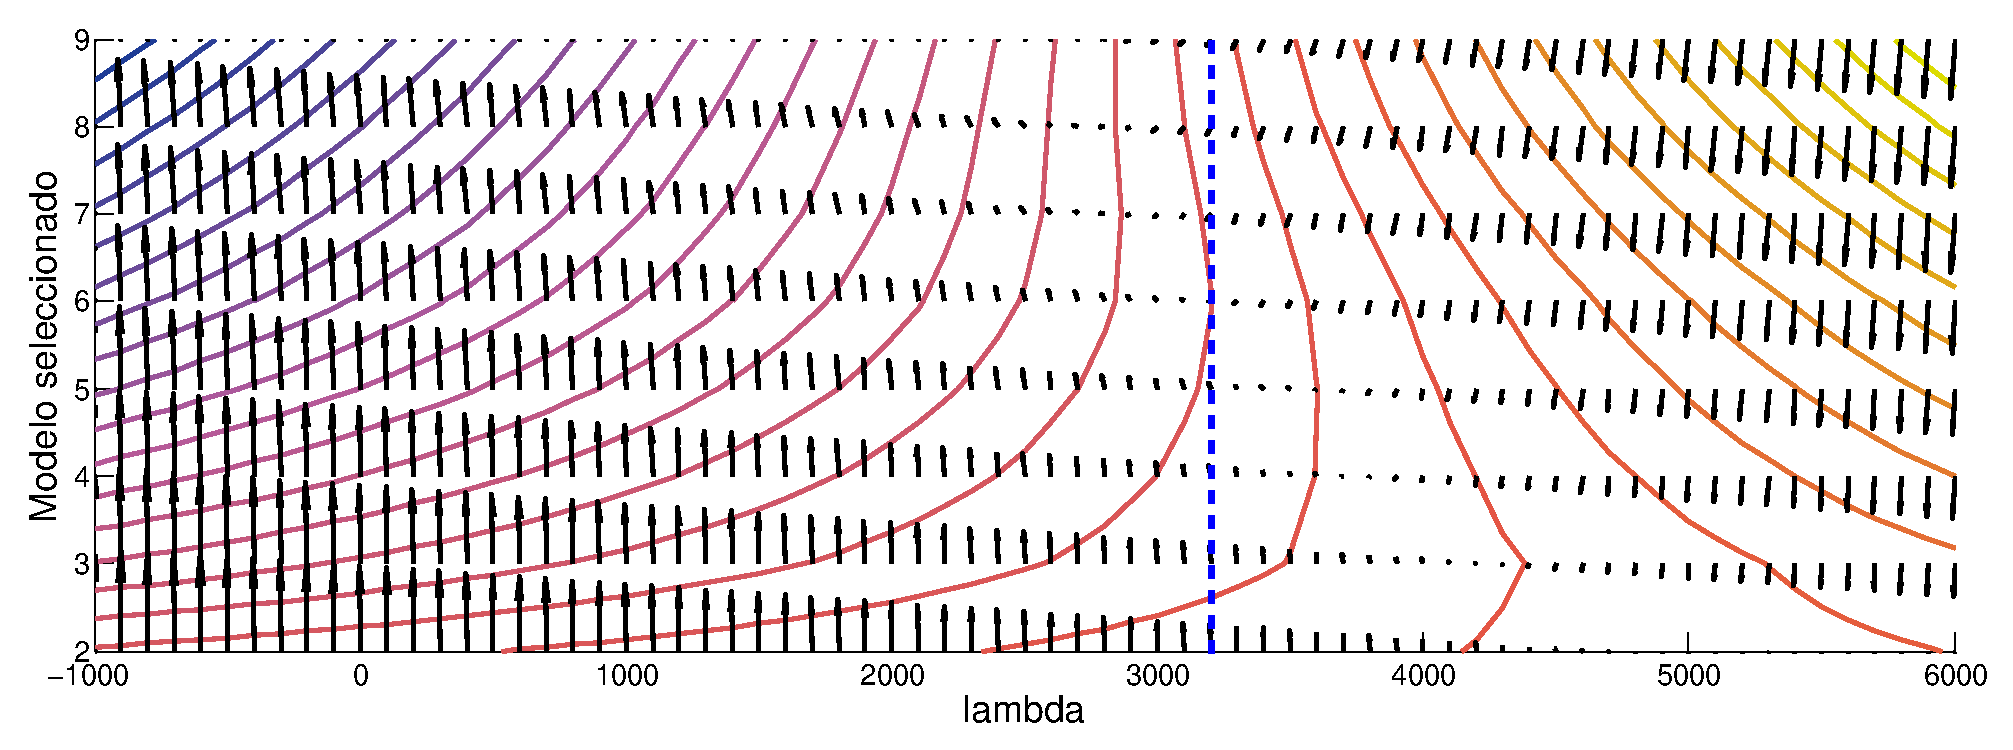
\includegraphics[width=1\textwidth]{gfx/chap6/cuervo1bic2}
   \caption{}
   \label{fig:seq1_bic2}
  \end{subfigure}  
  }  
  \centerline{
  \begin{subfigure}[b]{0.55\textwidth}
    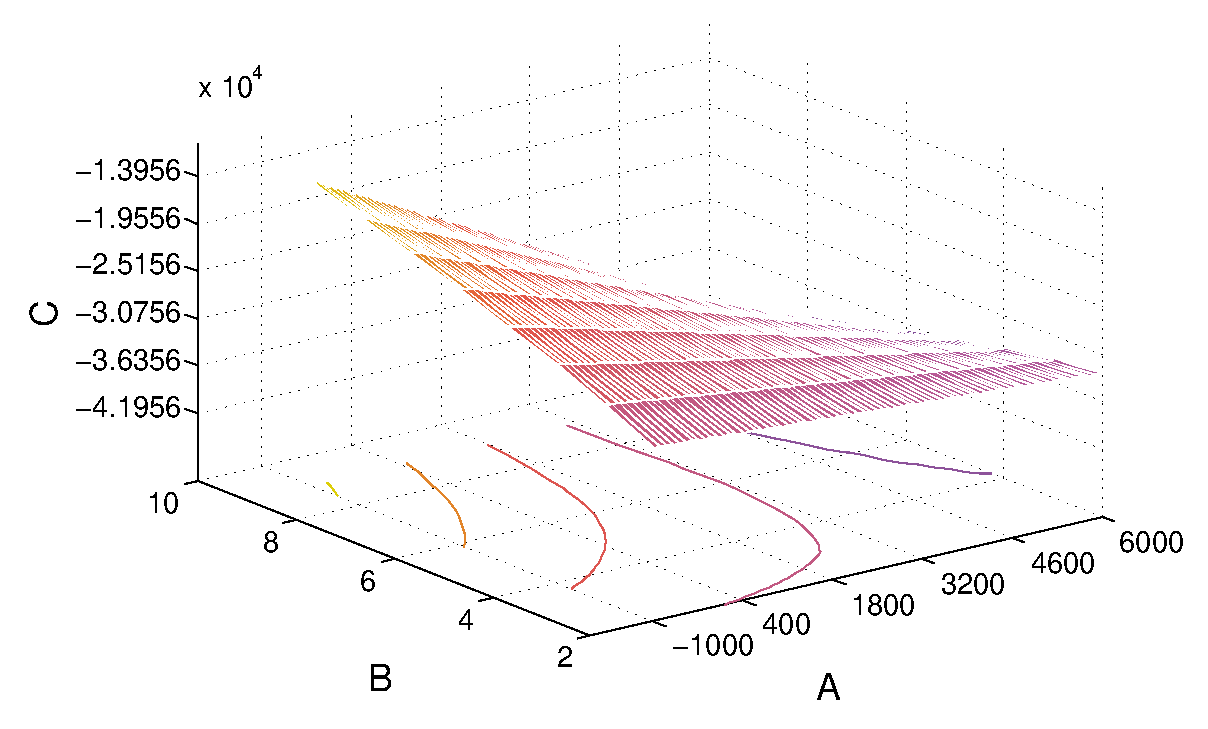
\includegraphics[width=\textwidth]{gfx/chap6/cuervo1bic1} 
    \caption{}
    \label{fig:seq1_bic1}
  \end{subfigure}  
  \begin{subfigure}[b]{0.55\textwidth}
    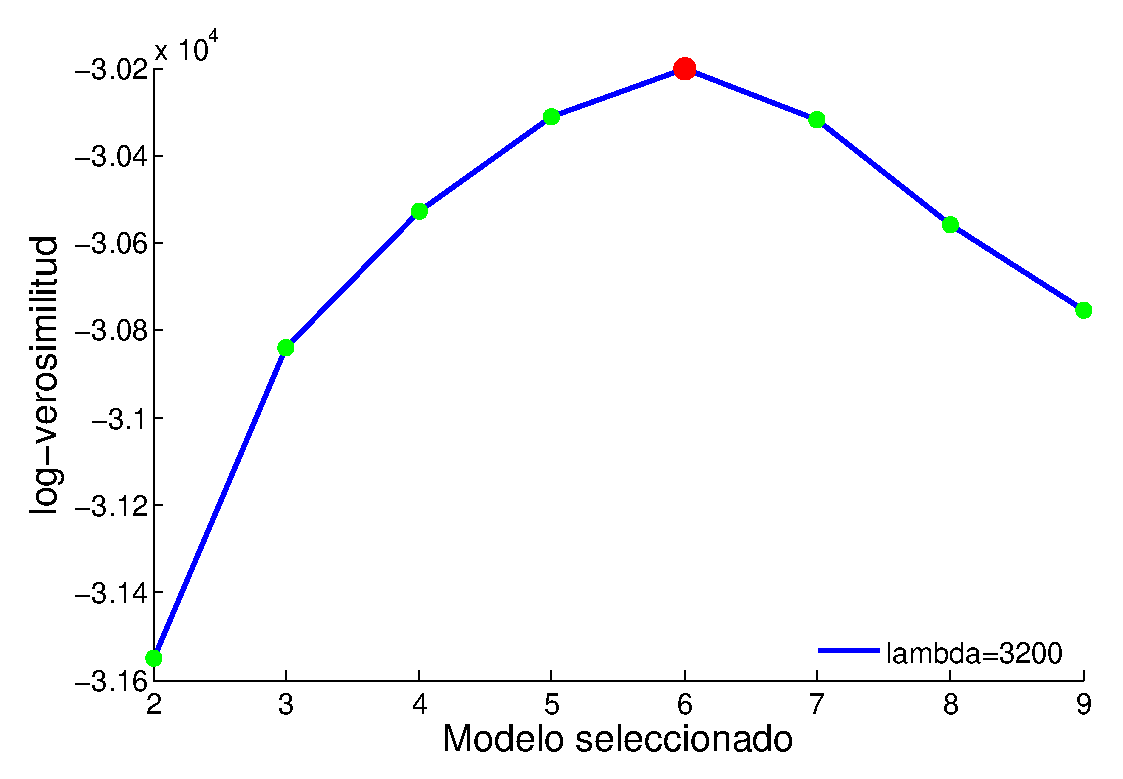
\includegraphics[width=\textwidth]{gfx/chap6/cuervo1bic3} 
    \caption{}
    \label{fig:seq1_bic3}
  \end{subfigure}
  }
  \caption[Secuencia 1: Pruebas BIC]{En la \autoref{fig:seq1_bic2}, se muestra las curvas de nivel de la superficie al variar el valor de lambda para evaluar BIC, así como la dirección del gradiente en la misma. En la \autoref{fig:seq1_bic1} se muestra una perspectiva general de superficie en \autoref{fig:seq1_bic2}. En la \autoref{fig:seq1_bic3} se muestra el valor seleccionado para lambda de acuerdo al análisis de sensibilidad realizado en la superficie anterior.}
  \label{fig:seq1_bic}
\end{figure}

En la \autoref{fig:seq1_bic1} se muestra la superficie generada al variar el valor de $\lambda$ para diferentes curvas de selección BIC. Se observa cómo al principio $\lambda$ es muy pequeño, y entonces el término de penalización no funciona por lo que se prefieren los modelos más complejos y sobre ajustados. Por otro lado, cuando $\lambda$ es muy grande, la penalización no permite mas que escoger los modelos más simples.

Haciendo un análisis de sensibilidad se puede determinar cuál es el parámetro $\lambda$ adecuado que penaliza de buena forma la log-verosimilitud.

En la \autoref{fig:seq1_bic2} se muestran las curvas de nivel de la figura anterior, además de la dirección del gradiente de la misma. Así mismo, en falso color se resaltan las zonas en las que el gradiente es menor. 

Lo que nos interesa encontrar en la superficie, es el valor de $\lambda$ que representa el punto de inflexión entre la selección de modelos demasiado complejos y modelos más simples. Para esto, se busca la zona en la que el gradiente sea lo más cercano a cero, pues implicaría que es un punto crítico.

Debido a la escala y a la forma en la que se calculó el gradiente, aunque para algunos valores cercanos de $\lambda$ no haya mucha variación en esa dirección; si \ac{BIC} está penalizando mal, entonces sí habrá gran variación para los diferentes modelos. Es por esto, que sólo en la zona en que la penalización sea del mismo orden de magnitud que la verosimilitud la variación en la curva \ac{BIC} con el $\lambda$ adecuado no será tan grande como en otras zonas.

Por último, se muestra en \autoref{fig:seq1_bic3} la curva BIC con el valor de $\lambda$ encontrado a partir del análisis de sensibilidad realizado en la \autoref{fig:seq1_bic2}. El o los modelos que tengan un mayor valor \ac{BIC} serán los que se seleccionarán como modelos ganadores.

\begin{figure}[t!]
  \centerline  
  { \begin{subfigure}[b]{0.7\textwidth}
      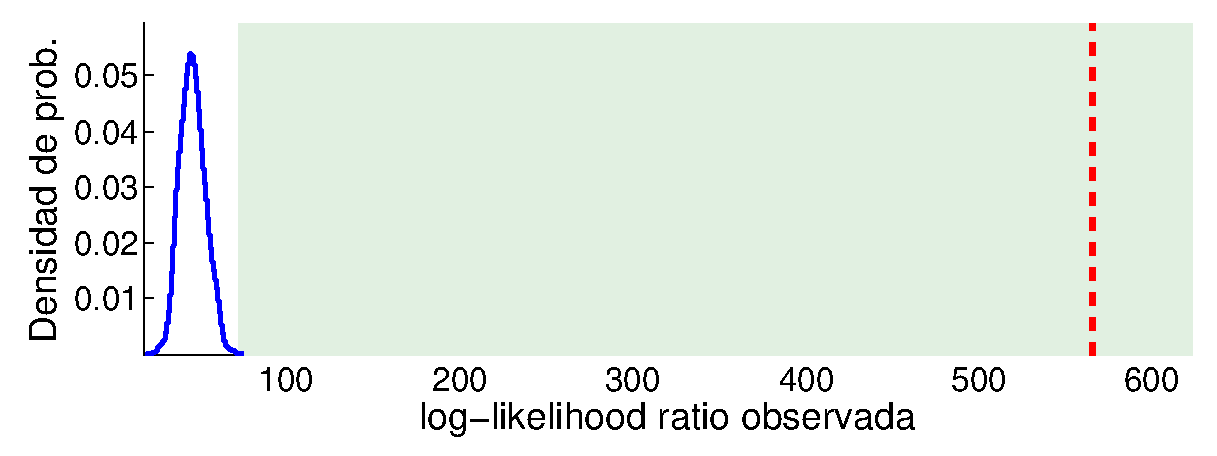
\includegraphics[width=1\linewidth]{gfx/chap6/cuervo1boot1}
      \caption{}
      \label{fig:seq1_boot1}
    \end{subfigure}
    \hspace{0.5cm}
    \begin{subfigure}[b]{0.7\textwidth}
      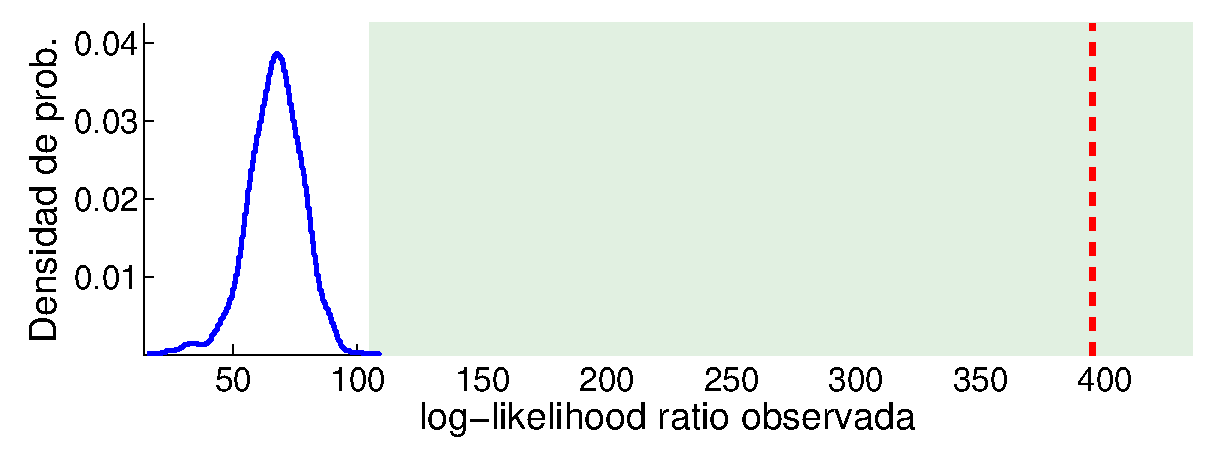
\includegraphics[width=1\linewidth]{gfx/chap6/cuervo1boot2}
      \caption{}
      \label{fig:seq1_boot2}
    \end{subfigure}
  }
  \centerline  
  { \begin{subfigure}[b]{0.7\textwidth}
      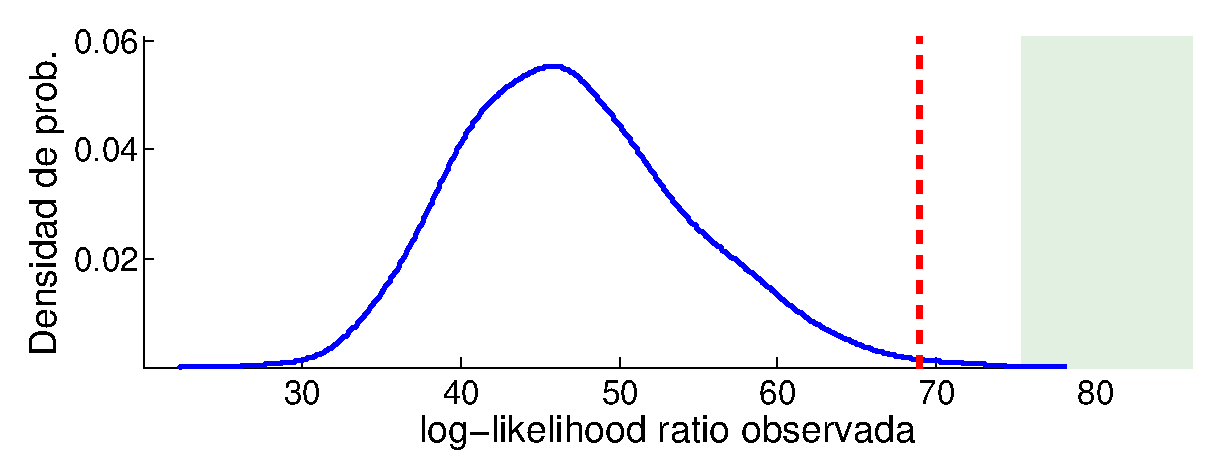
\includegraphics[width=1\linewidth]{gfx/chap6/cuervo1boot3}
      \caption{}
      \label{fig:seq1_boot3}
    \end{subfigure}
    \hspace{0.5cm}
    \begin{subfigure}[b]{0.7\textwidth}
      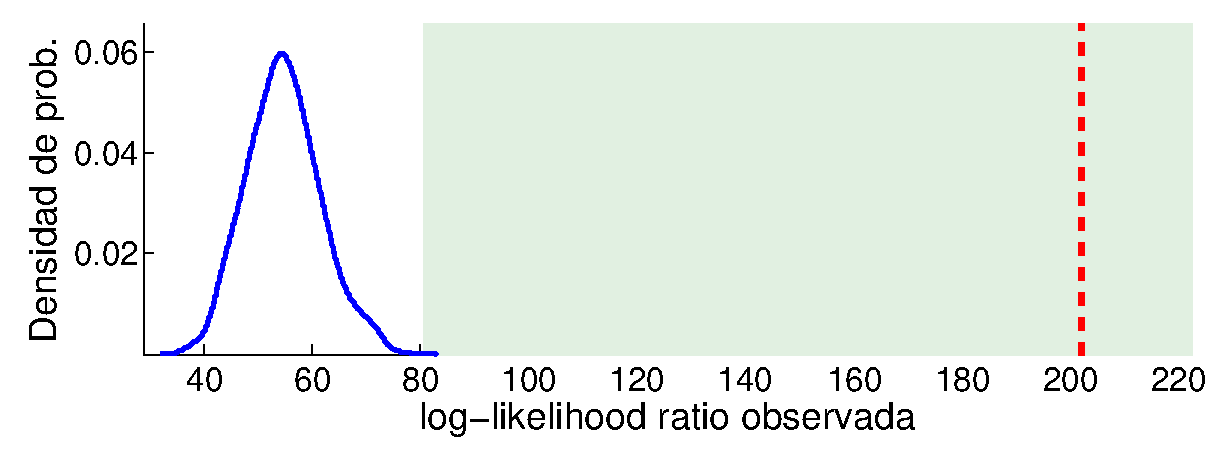
\includegraphics[width=1\linewidth]{gfx/chap6/cuervo1boot4}
      \caption{}
      \label{fig:seq1_boot4}
    \end{subfigure}
  }
  \caption[Secuencia 1: Pruebas de hipótesis usando bootstrap]{En la \autoref{fig:seq1_boot1} se muestra la prueba de hipótesis realizada para comparar el modelo $n_4$ contra $n_5$. Como se observa, se rechaza la hipótesis de que el modelo correcto sea $n_4$. En la \autoref{fig:seq1_boot2} se hace la prueba del modelo $n_5$ contra $n_6$, y de la misma manera, se rechaza la hipótesis de que el modelo correcto sea $n_5$. Se sigue con la prueba de hipótesis del modelo $n_6$ contra $n_7$ en la \autoref{fig:seq1_boot3}, y en este caso el valor observado no cae dentro de la región de rechazo, por lo que no podemos rechazar que el modelo $n_6$ sea el correcto. Por último en la \autoref{fig:seq1_boot4}, se hace la prueba del modelo $n_7$ contra el modelo $n_8$, y se vuelve a rechazar la hipótesis nula.}
  \label{fig:seq1_boot}
\end{figure}

En caso de que después de utilizar \ac{BIC} se presente ambigüedad para determinar un modelo ganador, o ya sea para realizar un análisis más exhaustivo, se puede propone hacer una prueba de hipótesis para determinar cuál modelo se ajusta mejor a los datos.

A diferencia de la primer etapa, en la que se usa \ac{BIC} como criterio para  seleccionar el mejor modelo de un conjunto no definido de modelos con diferentes parámetros, la intención de hacer pruebas de hipótesis es determinar en un pequeño conjunto de probables modelos, cuál es mejor, y qué tan bueno es un modelo respecto a otro.

Al plantear la prueba de hipótesis se harán una gran cantidad de simulaciones para ver qué tan bien se ajusta cada modelo a los datos originales, por lo que este proceso es computacionalmente intensivo y sólo se recomienda hacerlo para evitar la ambigüedad entre un par de modelos.

Por último, ya con el modelo seleccionado, se compara la segmentación recuperada con la secuencia o la segmentación originalde la conversación:
\begin{figure}[tp]
  \centerline
  {\begin{subfigure}[b]{1.3\textwidth}
      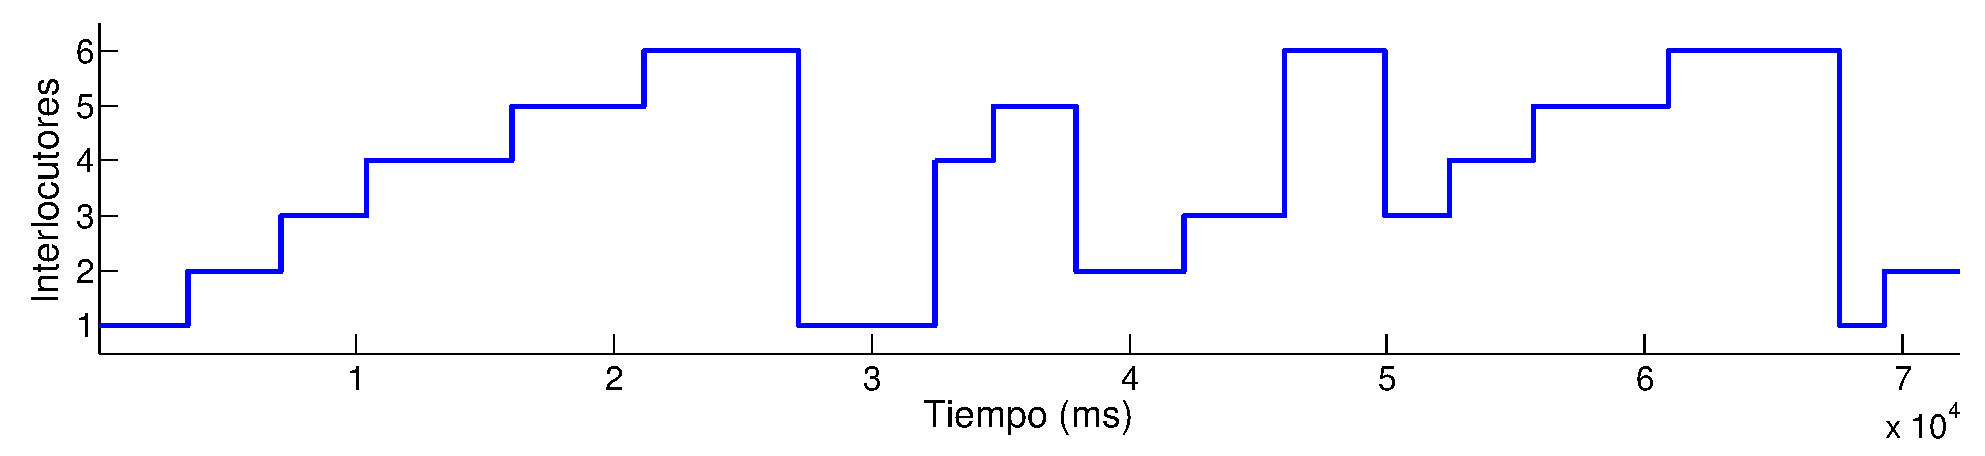
\includegraphics[width=1\linewidth]{gfx/chap6/cuervo1s_3_1}
      \caption{}
      \label{fig:seq1_seq1}
    \end{subfigure}
  } 
  \centerline
  {\begin{subfigure}[b]{1.3\textwidth}
      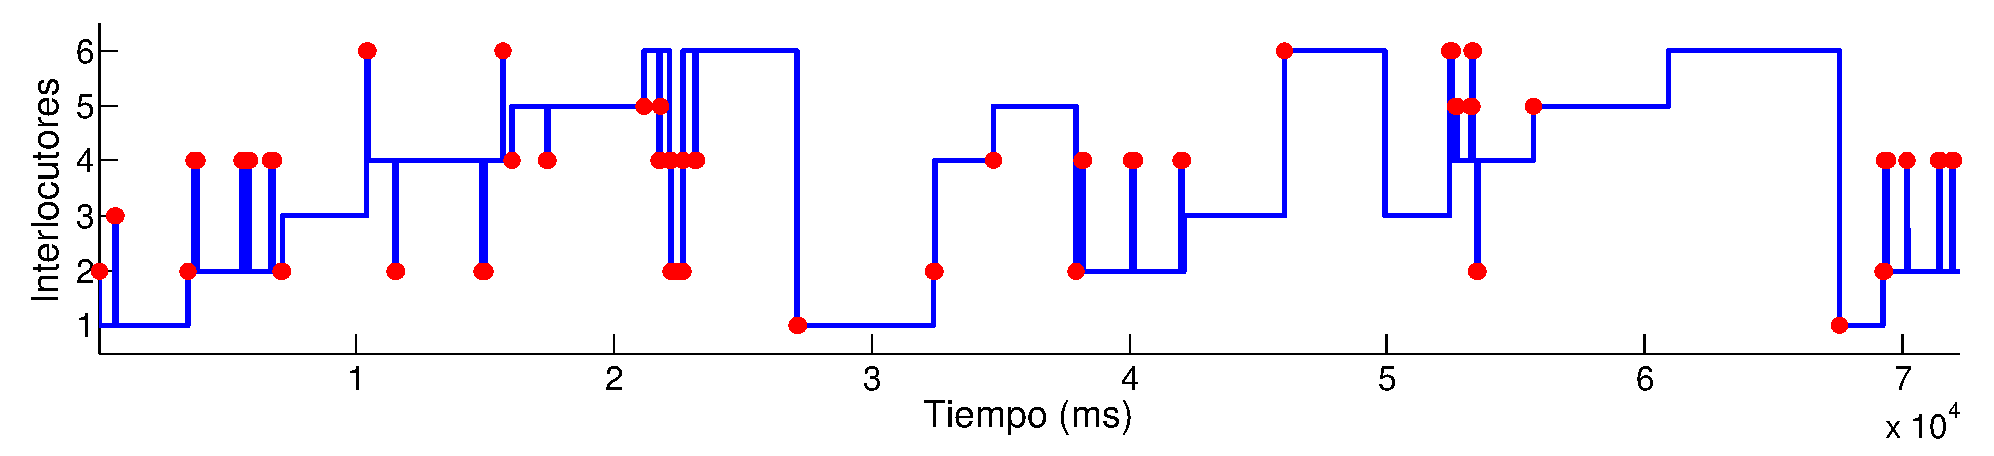
\includegraphics[width=1\linewidth]{gfx/chap6/cuervo1s_3_2}
      \caption{}
      \label{fig:seq1_seq2}
    \end{subfigure}
  }   
  \caption[Secuencia 1: Secuencia recuperada]{En \autoref{fig:seq1_seq1} se muestra la secuencia original de la \autoref{ssub:allanpoe}. En comparación, en \autoref{fig:seq1_seq2} se muestra la secuencia recuperada del modelo ganador y se marcan en rojo los errores cometidos respecto a la primera secuencia. }
  \label{fig:prb1_seq}
\end{figure}

Más a detalle, en la \autoref{fig:prb1_seq} se observa en azul el orden en el que participan los interlocutores de acuerdo a la secuencia recuperada. En rojo se marcan tanto los falsos positivos como los falsos negativos, de acuerdo al ground truth. 
Se observa también que la mayoría de las veces, en la secuencia recuperada se encuentran algunos brincos entre las personas, pero en esencia la estructura y el orden en que hablan los interlocutores es el correcto.
 

%%%%%%%%%%%%%%%%%%%%%%%%%%%%%%%%%%%%%%%%%%%%%%%%%%%%%%%%%%%%%%% 

\subsection[Secuencia 2]{Secuencia 2: Gabriel García Márquez} %(fold)
\label{ssub:soledad}

  Para la segunda secuencia se utilizaron algunos fragmentos de la novela 'El laberinto de la soledad' del escritor Gabriel García Márquez, con 4 distintas voces en español. La secuencia de audio original es de 6:55 min.

Para la etapa de agrupación de los vectores \ac{MFCC} con k-means++ se usaron 90 centros iniciales, mientras que el banco de filtros fue el mismo que en la secuencia anterior.

\begin{figure}[tp]
  \centerline{  
    \hspace{1.2cm}
    \parbox[c]{0.38\textwidth}{\centering Modelo generador}
    \parbox[c]{0.38\textwidth}{\centering Modelo $n_3$}
    \parbox[c]{0.38\textwidth}{\centering Modelo $n_4$}
    \parbox[c]{0.38\textwidth}{\centering Modelo $n_5$}
  }
  \vspace{0.5cm}
  \foreach \row in {1, ..., 2}{%  
    \centerline{%
      \parbox[c]{1cm}{
        \vspace{-0.5cm}
        \myheader{\row}
      }
      %\gdef \widthimg {0.35}
      \foreach \col in {1, ..., 4}{%
        \pgfmathparse{\col == 4 && \row == 2? 1:0}
        \ifthenelse{\pgfmathresult=1}{
          \gdef \widthimg {0.39}
        }{
          \gdef \widthimg {0.35}
        }
        \begin{subfigure}[c]{\widthimg \textwidth}          
          \def \imgfile {gfx/chap6/soledad1p_\col_\row}
          \IfFileExists{\imgfile.eps}{
            \includegraphics[width=1\textwidth]{\imgfile}
            \label{fig:seq2p_\col_\row}
          }{
            \hspace{1\textwidth}
          }
        \end{subfigure}
        %\hspace{-0.005\textwidth}
      }
    }
  }
\caption[Secuencia 2: Parámetros estimados (1)]{Por columnas, se muestran los parámetros obtenidos para varios modelos propuestos. La primer columna corresponde a los parámetros verdaderos.
En la primer fila \textup{(a)} se muestran las probabilidades a priori de que cada uno de los interlocutores empiecen la conversación. En la segunda fila \textup{(b)} se muestra en falso color la matriz de transición entre interlocutores para cada uno de los modelos mostrados.}
\label{fig:seq2p}
\end{figure}

En las \autoref{fig:seq2p} y \autoref{fig:seq2q} se muestran los parámetros estimados para los diferentes modelos que se propusieron. La primer columna corresponde a los parámetros verdaderos, mientras que las demás columnas son los parámetros obtenidos para diferentes modelos estimados. 

En la primer fila de la \autoref{fig:seq2p} se muestran las probabilidades a priori de que cada uno de los interlocutores empiecen el diálogo. En la segunda fila se muestra en falso color la matriz de transición para cada uno de los modelos. Esta matriz representa la probabilidad de cambio entre las personas que participan en la conversación.

De la misma manera, la matriz de transición que se recupera tiene estructura diagonal, como en la primer prueba.

\begin{figure}[t!]
  \centerline{
    \hspace{1.2cm}
    \parbox[c]{0.35\textwidth}{\centering Modelo generador}
    \parbox[c]{0.35\textwidth}{\centering Modelo $n_3$}
    \parbox[c]{0.35\textwidth}{\centering Modelo $n_4$}
    \parbox[c]{0.35\textwidth}{\centering Modelo $n_5$}
  }
  \vspace{0.5cm}
  \foreach \row in {3, ..., 7}{%  
    \centerline{
      \parbox[c]{1cm}{
        \vspace{-0.3cm}
        \myheader{\row}
      }
      \foreach \col in {1, ..., 4}{%
        \begin{subfigure}[c]{0.35\textwidth}  
          \def \imgfile {gfx/chap6/soledad1p_\col_\row}
          \IfFileExists{\imgfile.eps}{
            \includegraphics[width=1\textwidth]{\imgfile}
            %\caption{}
            \label{fig:seq2p_\col_\row}
          }{
            \hspace{1\textwidth}
          }
        \end{subfigure}
      }
    }
  }
\caption[Secuencia 2: Parámetros estimados (2)]{Por columnas, se muestran las probabilidades de emisión para cada uno de los interlocutores de acuerdo al modelo. Cada fila representa las probabilidad de emisión de las palabras en el diccionario. La fila \textup{(c)} para la primer persona, la fila \textup{(d)} para la segunda persona y así de forma consecutiva, de acuerdo al número de personas que contempla cada modelo propuesto.}
\label{fig:seq2q}
\end{figure}

En la \autoref{fig:seq2q} se muestran las probabilidades de emisión para cada uno de los participantes, de acuerdo a las palabras en las que se ha discretizado la conversación. Idealmente, cada interlocutor tiene asignadas con mayor probabilidad un cierto conjunto de palabras del diccionario, lo que hace que la identificación de las personas sea mucho más fácil de realizar.

Para la selección del modelo y como se explicó en el \autoref{ch:chap5}, primero se realiza una exploración del conjunto de posibles soluciones, por medio de \ac{BIC} regularizado para encontrar cuál o cuáles son los modelos más probables.

\begin{figure}[t!]
  \centerline{
  \begin{subfigure}[b]{1.1\textwidth}
   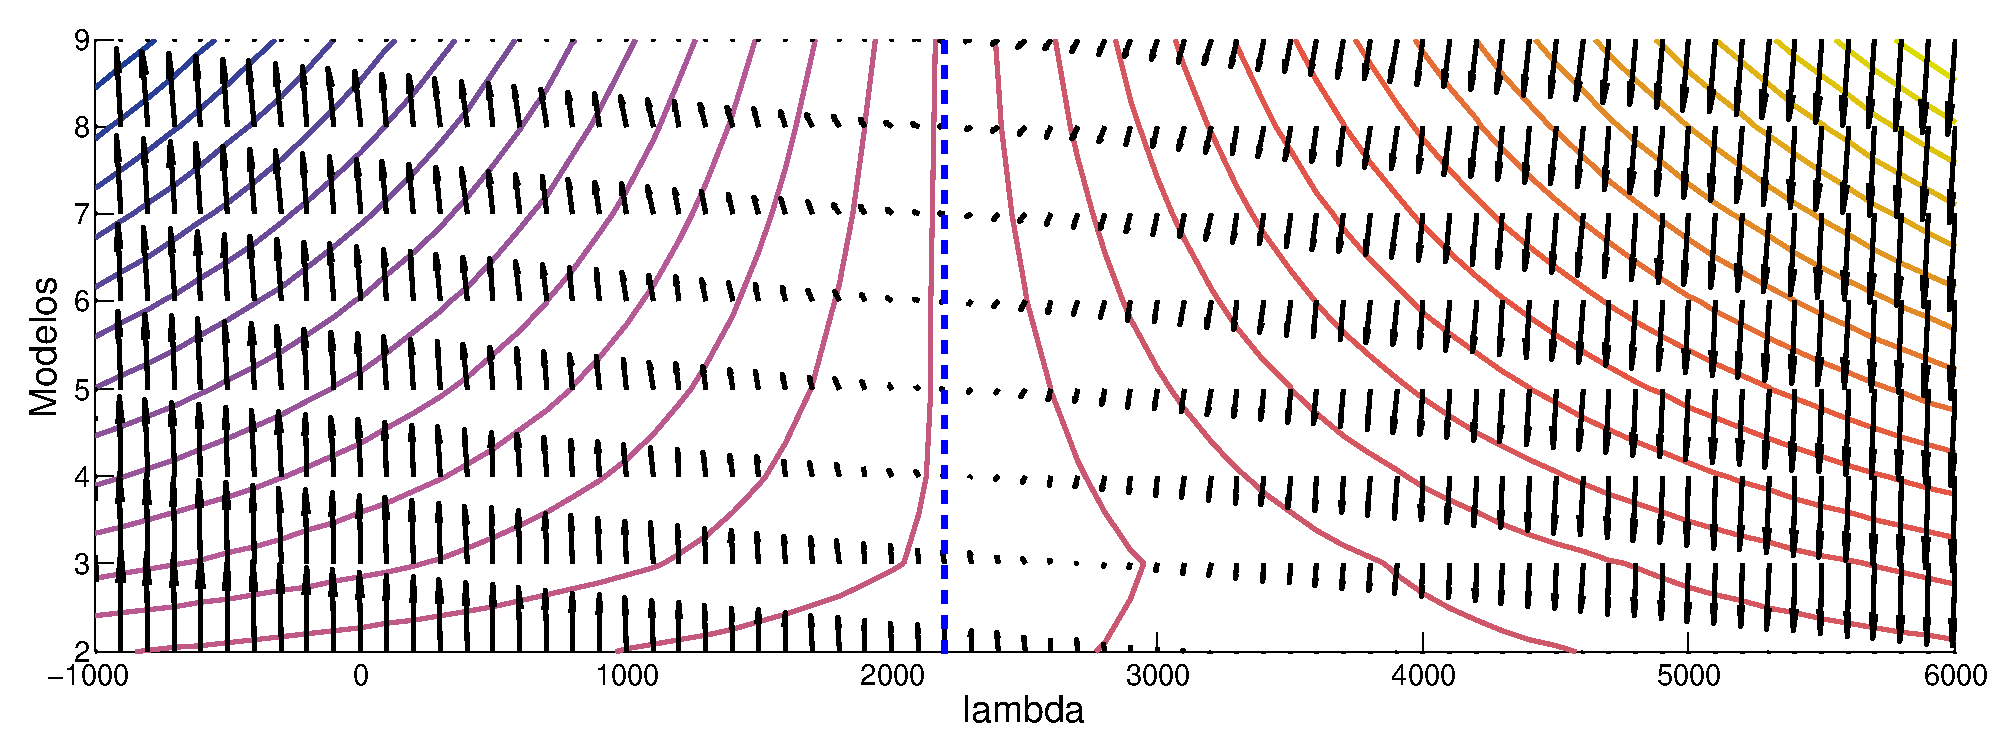
\includegraphics[width=1\textwidth]{gfx/chap6/calderon1bic2}
   \caption{}
   \label{fig:seq2_bic2}
  \end{subfigure}  
  }  
  \centerline{
  \begin{subfigure}[b]{0.55\textwidth}
    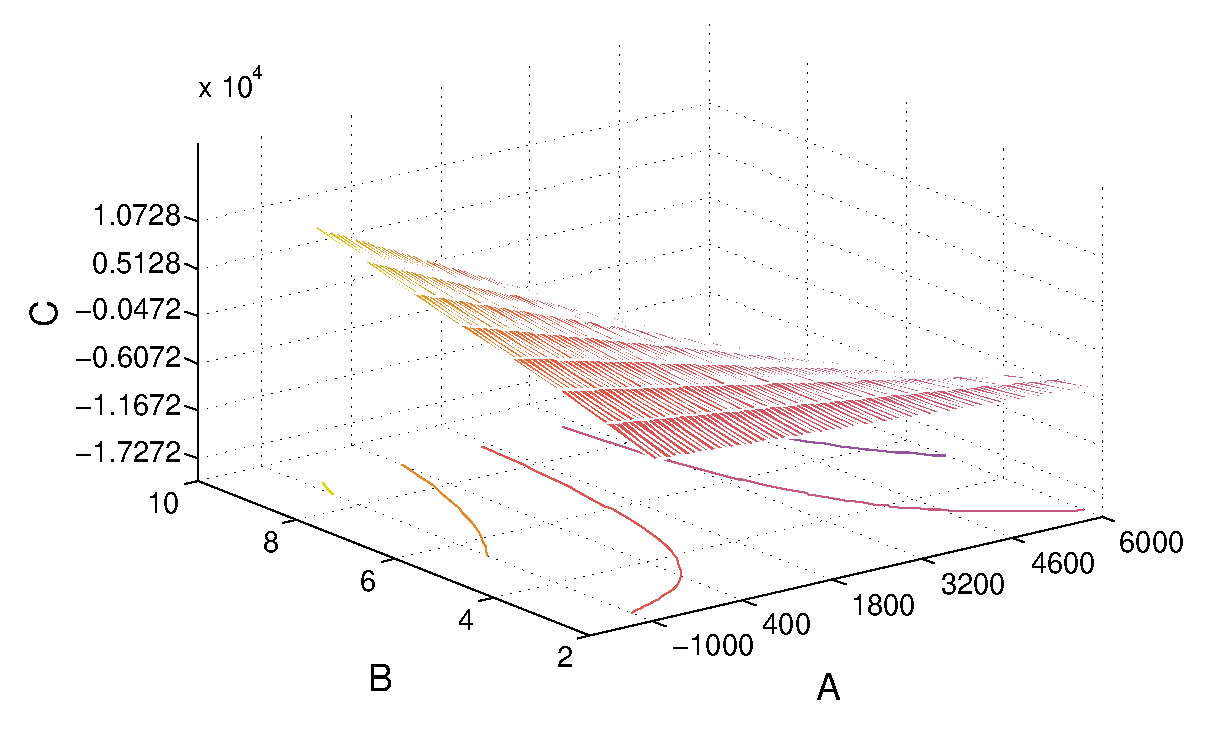
\includegraphics[width=\textwidth]{gfx/chap6/calderon1bic1} 
    \caption{}
    \label{fig:seq2_bic1}
  \end{subfigure}  
  \begin{subfigure}[b]{0.55\textwidth}
    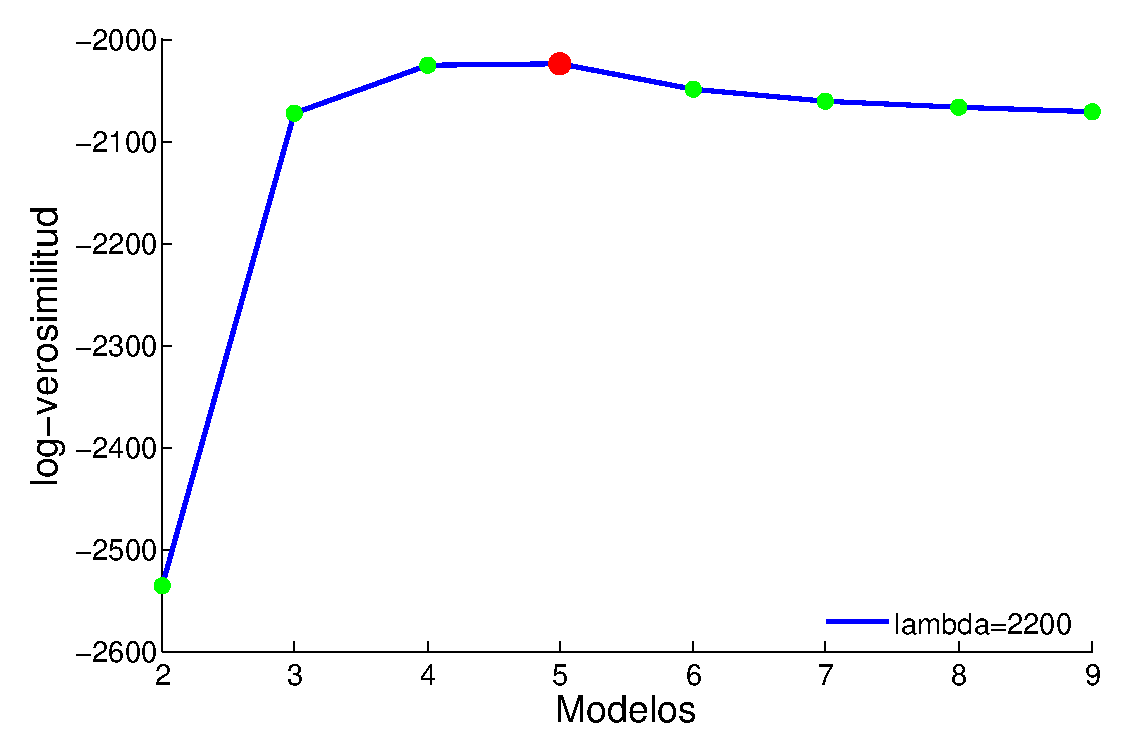
\includegraphics[width=\textwidth]{gfx/chap6/calderon1bic3} 
    \caption{}
    \label{fig:seq2_bic3}
  \end{subfigure}
  }
  \caption[Secuencia 2: Pruebas BIC]{En la \autoref{fig:seq2_bic2}, se muestra las curvas de nivel de la superficie al variar el valor de lambda para evaluar BIC, así como la dirección del gradiente en la misma. En la \autoref{fig:seq2_bic1} se muestra una perspectiva general de superficie en \autoref{fig:seq2_bic2}. En la \autoref{fig:seq2_bic3} se muestra el valor seleccionado para lambda de acuerdo al análisis de sensibilidad realizado en la superficie anterior.}
  \label{fig:seq2_bic}
\end{figure}

En la \autoref{fig:seq2_bic1} se muestra la superficie generada al variar el valor de $\lambda$ para diferentes curvas de selección \ac{BIC}. Haciendo un análisis de sensibilidad se puede determinar cuál es el parámetro $\lambda$ adecuado que penaliza de buena forma la log-verosimilitud. En la \autoref{fig:seq2_bic2} se muestran las curvas de nivel de la figura anterior, además de la dirección del gradiente de la misma. Así mismo, en falso color se resaltan las zonas en las que el gradiente es menor. 

Por último, se muestra en \autoref{fig:seq2_bic3} la curva \ac{BIC} con el valor de $\lambda$ encontrado a partir del análisis de sensibilidad realizado en la \autoref{fig:seq2_bic2}. El o los modelos que tengan un mayor valor \ac{BIC} serán los que se seleccionarán como modelos ganadores.

\begin{figure}[t!]
  \centerline  
  { \begin{subfigure}[b]{0.7\textwidth}
      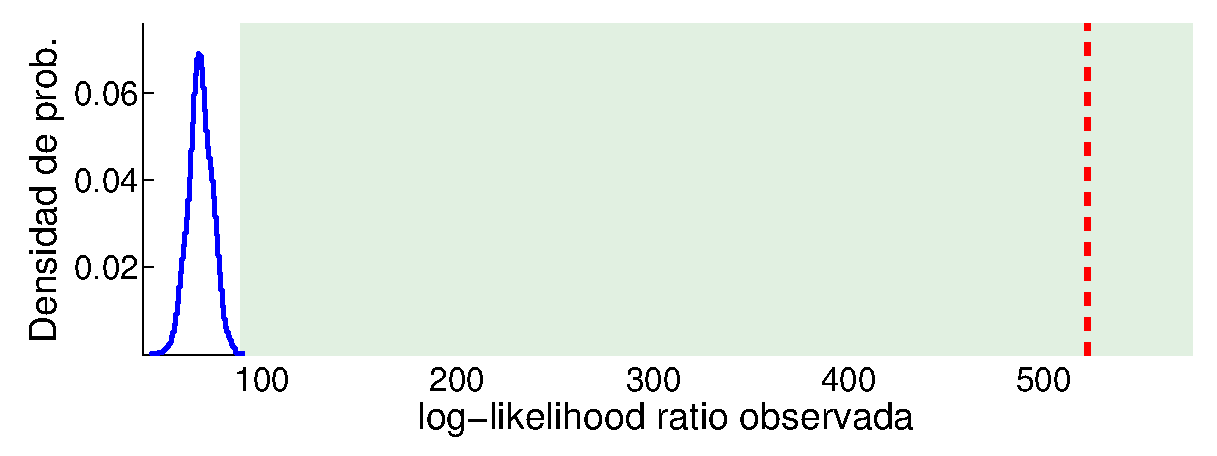
\includegraphics[width=1\linewidth]{gfx/chap6/soledad1boot1}
      \caption{}
      \label{fig:seq2_boot1}
    \end{subfigure}
    \hspace{0.5cm}
    \begin{subfigure}[b]{0.7\textwidth}
      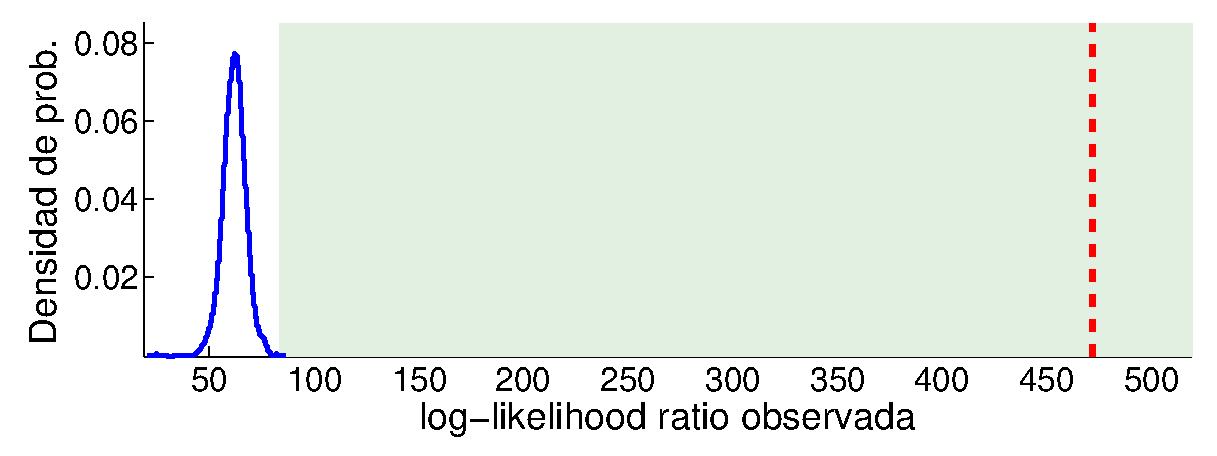
\includegraphics[width=1\linewidth]{gfx/chap6/soledad1boot2}
      \caption{}
      \label{fig:seq2_boot2}
    \end{subfigure}
  }
  \centerline  
  { \begin{subfigure}[b]{0.7\textwidth}
      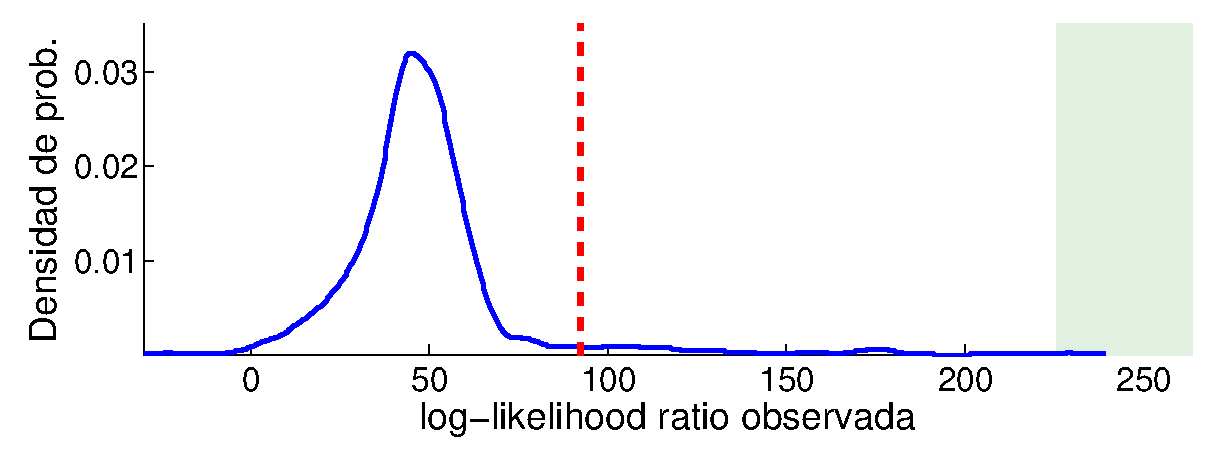
\includegraphics[width=1\linewidth]{gfx/chap6/soledad1boot3}
      \caption{}
      \label{fig:seq2_boot3}
    \end{subfigure}
    \hspace{0.5cm}
    \begin{subfigure}[b]{0.7\textwidth}
      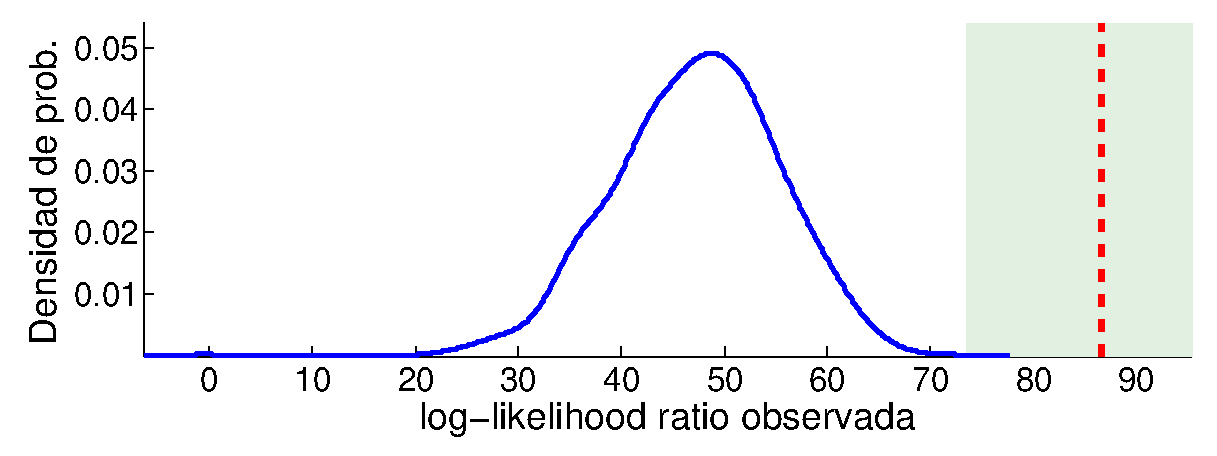
\includegraphics[width=1\linewidth]{gfx/chap6/soledad1boot4}
      \caption{}
      \label{fig:seq2_boot4}
    \end{subfigure}
  }
  \caption[Secuencia 2: Pruebas de hipótesis usando bootstrap]{En la \autoref{fig:seq2_boot1} se muestra la prueba de hipótesis realizada para comparar el modelo $n_2$ contra $n_3$. Como se observa, se rechaza la hipótesis de que el modelo correcto sea $n_4$. En la \autoref{fig:seq2_boot2} se hace la prueba del modelo $n_3$ contra $n_4$, y de la misma manera, se rechaza la hipótesis de que el modelo correcto sea $n_3$. Se sigue con la prueba de hipótesis del modelo $n_4$ contra $n_5$ en la \autoref{fig:seq2_boot3}, y en este caso el valor observado no cae dentro de la región de rechazo, por lo que no podemos rechazar que el modelo $n_4$ sea el correcto. Por último en la \autoref{fig:seq2_boot4}, se hace la prueba del modelo $n_5$ contra el modelo $n_6$, y se vuelve a rechazar la hipótesis nula.}  
  \label{fig:seq2_boot}
\end{figure}

En caso de que después de utilizar BIC se presente ambigüedad para determinar un modelo ganador, o ya sea para realizar un análisis más exhaustivo, se puede propone hacer una prueba de hipótesis para determinar cuál modelo se ajusta mejor a los datos.

A diferencia de la primer etapa, en la que se usa BIC como criterio para  seleccionar el mejor modelo de un conjunto no definido de modelos con diferentes parámetros, la intención de hacer pruebas de hipótesis es determinar en un pequeño conjunto de probables modelos, cuál es mejor, y qué tan bueno es un modelo respecto a otro.

Al plantear la prueba de hipótesis se harán una gran cantidad de simulaciones para ver qué tan bien se ajusta cada modelo a los datos originales, por lo que este proceso es computacionalmente intensivo y sólo se recomienda hacerlo para evitar la ambigüedad entre un par de modelos.

...

Por último, ya con el modelo seleccionado, se procede a calcular el error relativo de predicción que se obtuvo, comparando con el ground truth que se dispone para esa secuencia, con lo que se obtiene: 

...

\begin{figure}[tp]
  \centerline
  {\begin{subfigure}[b]{1.3\textwidth}
      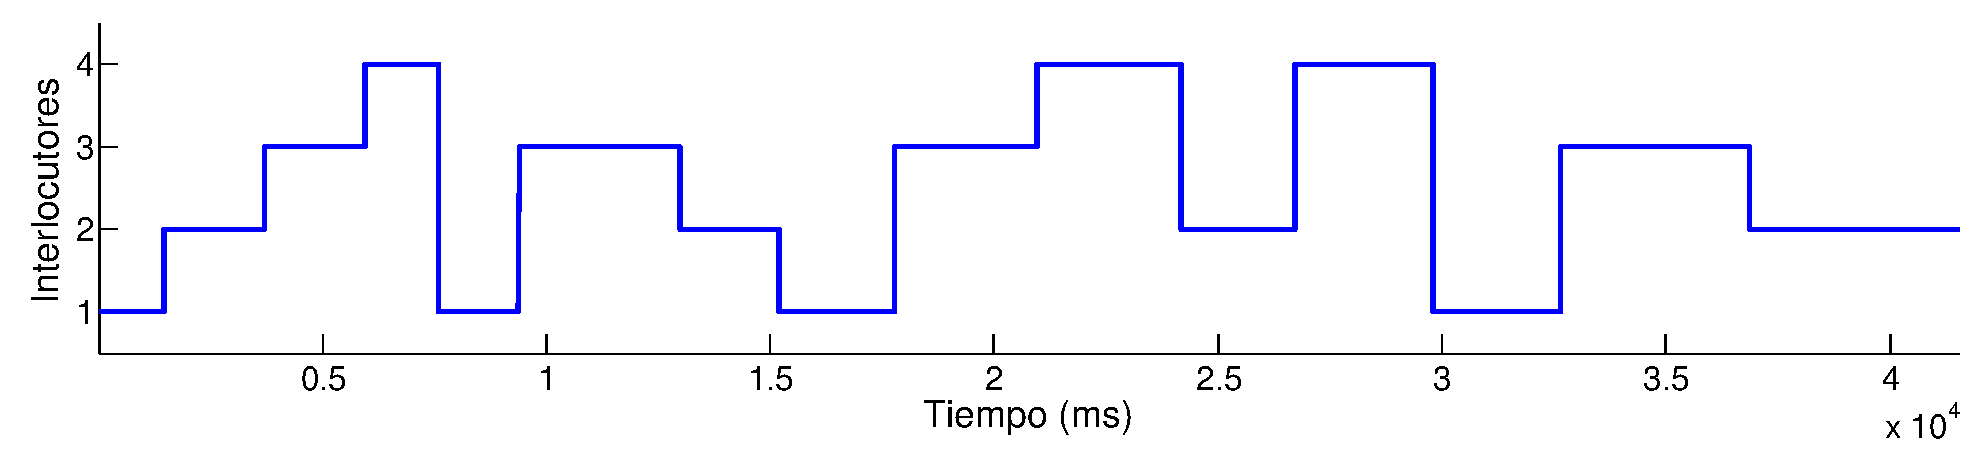
\includegraphics[width=1\linewidth]{gfx/chap6/soledad1s_3_1}
      \caption{}
      \label{fig:seq2_seq1}
    \end{subfigure}
  } 
  \centerline
  {\begin{subfigure}[b]{1.3\textwidth}
      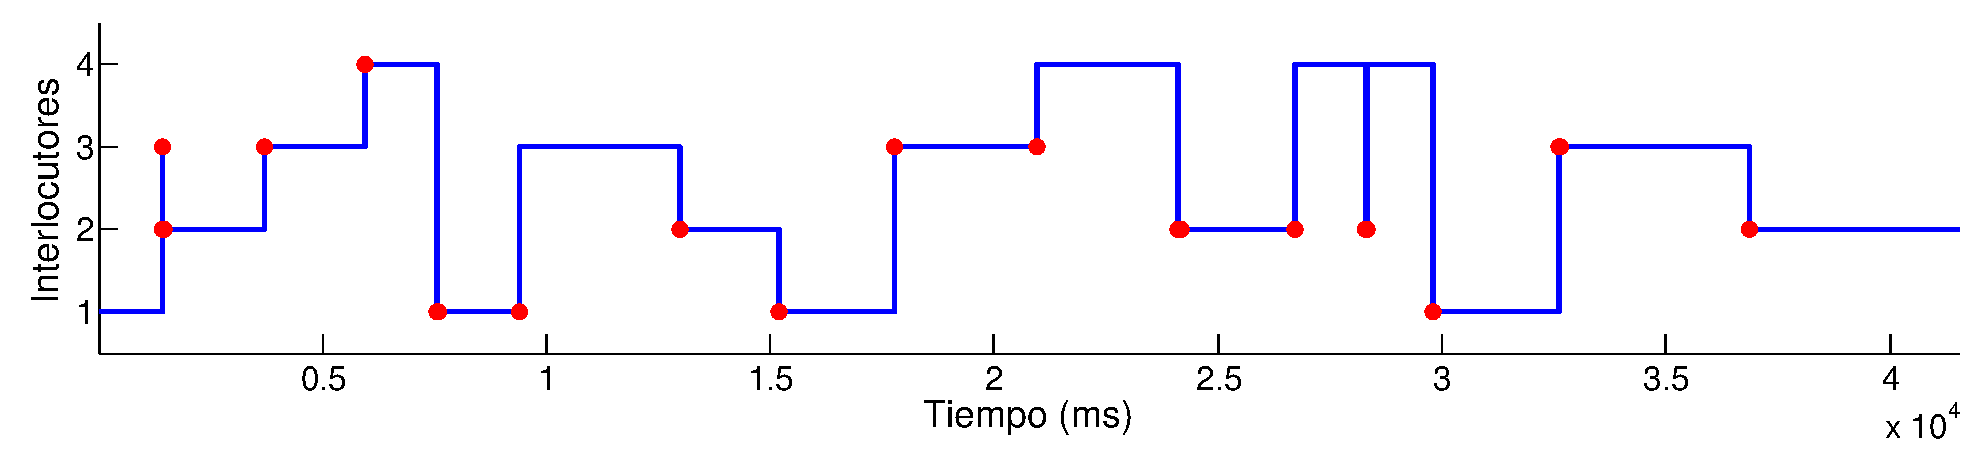
\includegraphics[width=1\linewidth]{gfx/chap6/soledad1s_3_2}
      \caption{}
      \label{fig:seq2_seq2}
    \end{subfigure}
  }
  \caption[Secuencia 2: Secuencia recuperada]{En \autoref{fig:seq2_seq1} se muestra la secuencia original de la \autoref{ssub:soledad}. En comparación, en \autoref{fig:seq2_seq2} se muestra la secuencia recuperada del modelo ganador y se marcan en rojo los errores cometidos respecto a la primera secuencia. }
  \label{fig:prb2_seq}
\end{figure}

Más a detalle, en la \autoref{fig:prb2_seq} se observa en azul el orden en el que participan los interlocutores de acuerdo a la secuencia recuperada. En rojo se marcan tanto los falsos positivos como los falsos negativos, de acuerdo al ground truth. Hay que notar que cuando el número de estados para un modelo no es el correcto, entonces inminentemente el número de errores en la secuencia obtenida será mayor, pues al menos todas las intervenciones de un hablante no podrán ser emparejadas o serán asignadas a alguien más.

Se observa también que la mayoría de las veces, en la secuencia recuperada se encuentran algunos brincos entre personas, pero en esencia la estructura y el orden en que hablan los interlocutores es el correcto. 

%%%%%%%%%%%%%%%%%%%%%%%%%%%%%%%%%%%%%%%%%%%%%%%%%%%%%%%%%%%%%%% 

\subsection[Secuencia 3]{Secuencia 3: William Shakespeare}
\label{ssub:lear}

  Para esta secuencia se utilizaron algunos poemas del escritor William Shakespeare, alternando 6 voces diferentes en inglés. La secuencia de audio original tiene una duración de 12:01 min.

Para la etapa de agrupación de los vectores MFCC con k-means++ se usaron 140 centros iniciales, mientras que el banco de filtros fue el mismo que en la secuencia anterior.

\begin{figure}[tp]
  \centerline{  
    \hspace{1.2cm}
    \parbox[c]{0.38\textwidth}{\centering Modelo generador}
    \parbox[c]{0.38\textwidth}{\centering Modelo $n_5$}
    \parbox[c]{0.38\textwidth}{\centering Modelo $n_6$}
    \parbox[c]{0.38\textwidth}{\centering Modelo $n_7$}
  }
  \vspace{0.5cm}
  \foreach \row in {1, ..., 2}{%  
    \centerline{%
      \parbox[c]{1cm}{
        \vspace{-0.5cm}
        \myheader{\row}
      }
      %\gdef \widthimg {0.35}
      \foreach \col in {1, ..., 4}{%
        \pgfmathparse{\col == 4 && \row == 2? 1:0}
        \ifthenelse{\pgfmathresult=1}{
          \gdef \widthimg {0.39}
        }{
          \gdef \widthimg {0.35}
        }
        \begin{subfigure}[c]{\widthimg \textwidth}          
          \def \imgfile {gfx/chap6/lear3p_\col_\row}
          \IfFileExists{\imgfile.eps}{
            \includegraphics[width=1\textwidth]{\imgfile}
            \label{fig:seq3p_\col_\row}
          }{
            \hspace{1\textwidth}
          }
        \end{subfigure}
        %\hspace{-0.005\textwidth}
      }
    }
  }
\caption[Secuencia 3: Parámetros estimados (1)]{Por columnas, se muestran los parámetros obtenidos para varios modelos propuestos. La primer columna corresponde a los parámetros verdaderos.
En la primer fila \textup{(a)} se muestran las probabilidades a priori de que cada uno de los interlocutores empiecen la conversación. En la segunda fila \textup{(b)} se muestra en falso color la matriz de transición entre interlocutores para cada uno de los modelos mostrados.}
\label{fig:seq3p}
\end{figure}

En las \autoref{fig:seq3p} y \autoref{fig:seq3q} se muestran los parámetros estimados para los diferentes modelos que se propusieron. La primer columna corresponde a los parámetros verdaderos, mientras que las demás columnas son los parámetros obtenidos para diferentes modelos estimados. 

En la primer fila de la \autoref{fig:seq3p} se muestran las probabilidades a priori de que cada uno de los interlocutores empiecen el diálogo. En la segunda fila se muestra en falso color la matriz de transición para cada uno de los modelos. Esta matriz representa la probabilidad de cambio entre las personas que participan en la conversación.

Se observa como en general para todos los modelos propuestos la matriz de transición que se recupera tiene una estructura diagonal, puesto que en este tipo de problemas, una persona suele hablar durante un periodo considerablemente largo, para que luego otra persona empiece a hablar.

\begin{figure}[t!]
  \centerline{
    \hspace{1.2cm}
    \parbox[c]{0.35\textwidth}{\centering Modelo generador}
    \parbox[c]{0.35\textwidth}{\centering Modelo $n_5$}
    \parbox[c]{0.35\textwidth}{\centering Modelo $n_6$}
    \parbox[c]{0.35\textwidth}{\centering Modelo $n_7$}
  }
  \vspace{0.5cm}
  \foreach \row in {3, ..., 7}{%  
    \centerline{
      \parbox[c]{1cm}{
        \vspace{-0.3cm}
        \myheader{\row}
      }
      \foreach \col in {1, ..., 4}{%
        \begin{subfigure}[c]{0.35\textwidth}  
          \def \imgfile {gfx/chap6/lear3p_\col_\row}
          \IfFileExists{\imgfile.eps}{
            \includegraphics[width=1\textwidth]{\imgfile}
            %\caption{}
            \label{fig:seq3p_\col_\row}
          }{
            \hspace{1\textwidth}
          }
        \end{subfigure}
      }
    }
  }
\caption[Secuencia 3: Parámetros estimados (2)]{Por columnas, se muestran las probabilidades de emisión para cada uno de los interlocutores de acuerdo al modelo. Cada fila representa las probabilidad de emisión de las palabras en el diccionario. La fila \textup{(c)} para la primer persona, la fila \textup{(d)} para la segunda persona y así de forma consecutiva, de acuerdo al número de personas que contempla cada modelo propuesto.}
\label{fig:seq3q}
\end{figure}

En la \autoref{fig:seq3q} se muestran las probabilidades de emisión para cada uno de los participantes, de acuerdo a las palabras en las que se ha discretizado la conversación. Idealmente, cada interlocutor tiene asignadas con mayor probabilidad un cierto conjunto de palabras del diccionario, lo que hace que la identificación de las personas sea mucho más fácil de realizar.

Para la selección del modelo y siguiendo la metodología propuesta, primero se efectúa una inspección por medio de BIC regularizado para encontrar cuál o cuáles son los modelos más probables.

\begin{figure}[t!]
  \centerline{
  \begin{subfigure}[b]{1.1\textwidth}
   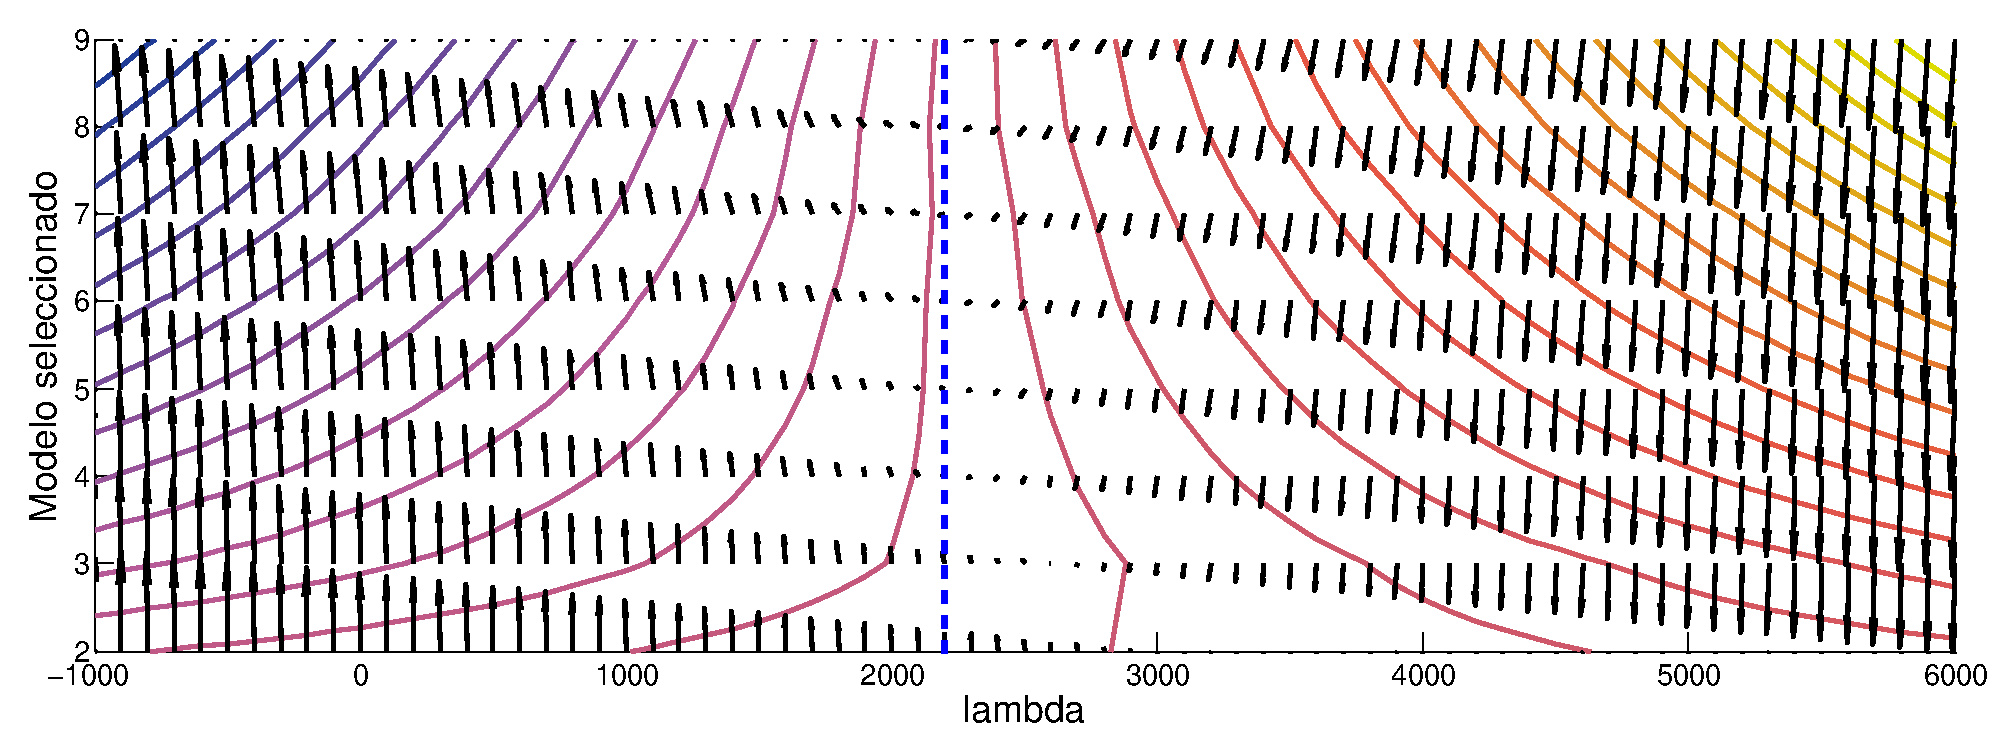
\includegraphics[width=1\textwidth]{gfx/chap6/lear3bic2}
   \caption{}
   \label{fig:seq3_bic2}
  \end{subfigure}  
  }  
  \centerline{
  \begin{subfigure}[b]{0.55\textwidth}
    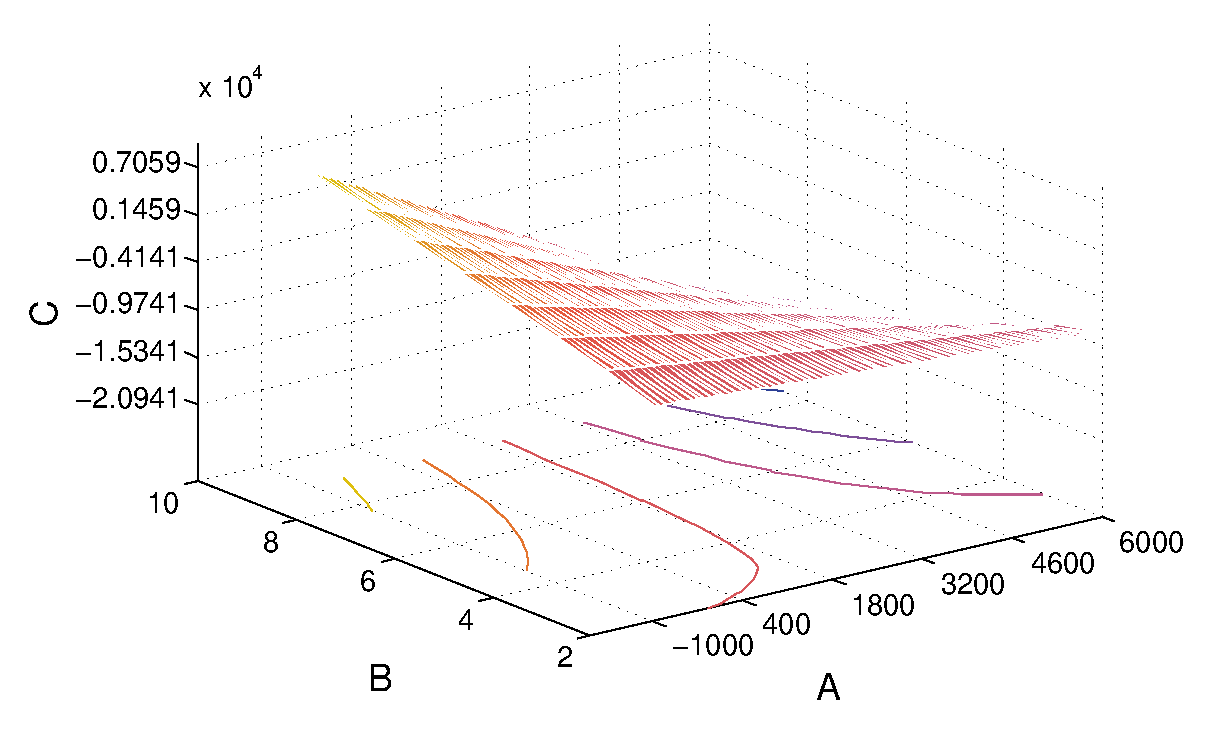
\includegraphics[width=\textwidth]{gfx/chap6/lear3bic1} 
    \caption{}
    \label{fig:seq3_bic1}
  \end{subfigure}  
  \begin{subfigure}[b]{0.55\textwidth}
    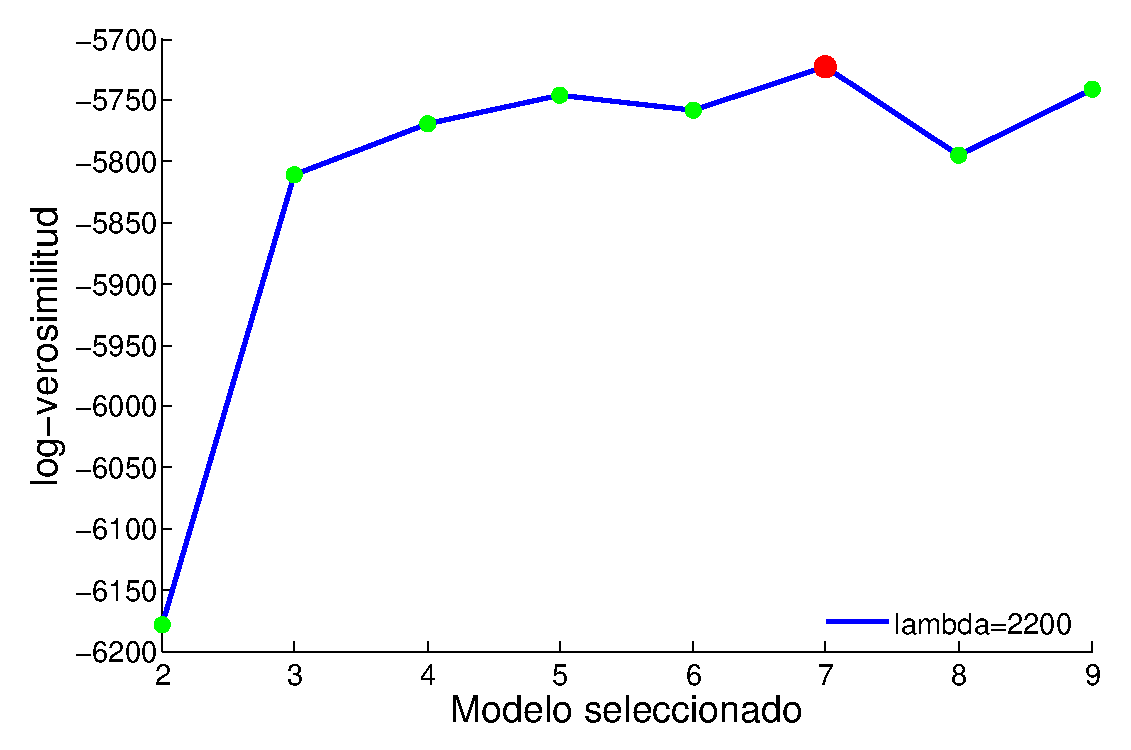
\includegraphics[width=\textwidth]{gfx/chap6/lear3bic3} 
    \caption{}
    \label{fig:seq3_bic3}
  \end{subfigure}
  }
  \caption[Secuencia 3: Pruebas BIC]{En la \autoref{fig:seq3_bic2}, se muestra las curvas de nivel de la superficie al variar el valor de lambda para evaluar BIC, así como la dirección del gradiente en la misma. En la \autoref{fig:seq3_bic1} se muestra una perspectiva general de superficie en \autoref{fig:seq3_bic2}. En la \autoref{fig:seq3_bic3} se muestra el valor seleccionado para lambda de acuerdo al análisis de sensibilidad realizado en la superficie anterior.}
  \label{fig:seq1_bic}
\end{figure}

En la \autoref{fig:seq3_bic1} se muestra la superficie generada al variar el valor de $\lambda$ para diferentes curvas de selección BIC. Se observa cómo al principio $\lambda$ es muy pequeño, y entonces el término de penalización no funciona por lo que se prefieren los modelos más complejos y sobre ajustados. Por otro lado, cuando $\lambda$ es muy grande, la penalización no permite mas que escoger los modelos más simples.

Haciendo un análisis de sensibilidad se puede determinar cuál es el parámetro $\lambda$ adecuado que penaliza de buena forma la log-verosimilitud.

En la \autoref{fig:seq3_bic2} se muestran las curvas de nivel de la figura anterior, además de la dirección del gradiente de la misma. Así mismo, en falso color se resaltan las zonas en las que el gradiente es menor. 

Lo que nos interesa encontrar en la superficie, es el valor de $\lambda$ que representa el punto de inflexión entre la selección de modelos demasiado complejos y modelos más simples. Para esto, se busca la zona en la que el gradiente sea lo más cercano a cero, pues implicaría que es un punto crítico.

Debido a la escala y a la forma en la que se calculó el gradiente, aunque para algunos valores cercanos de $\lambda$ no haya mucha variación en esa dirección; si BIC está penalizando mal, entonces sí habrá gran variación para los diferentes modelos. Es por esto, que sólo en la zona en que la penalización sea del mismo orden de magnitud que la verosimilitud la variación en la curva BIC con el $\lambda$ adecuado no será tan grande como en otras zonas.

Por último, se muestra en \autoref{fig:seq3_bic3} la curva BIC con el valor de $\lambda$ encontrado a partir del análisis de sensibilidad realizado en la \autoref{fig:seq3_bic2}. El o los modelos que tengan un mayor valor BIC serán los que se seleccionarán como modelos ganadores.

\begin{figure}[t!]
  \centerline  
  { \begin{subfigure}[b]{0.7\textwidth}
      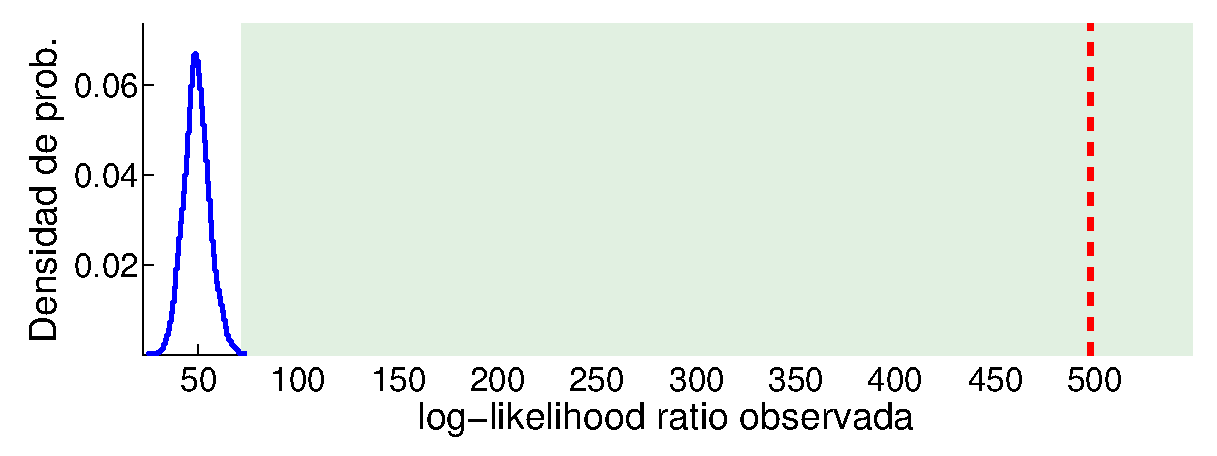
\includegraphics[width=1\linewidth]{gfx/chap6/lear3boot1}
      \caption{}
      \label{fig:seq3_boot1}
    \end{subfigure}
    \hspace{0.5cm}
    \begin{subfigure}[b]{0.7\textwidth}
      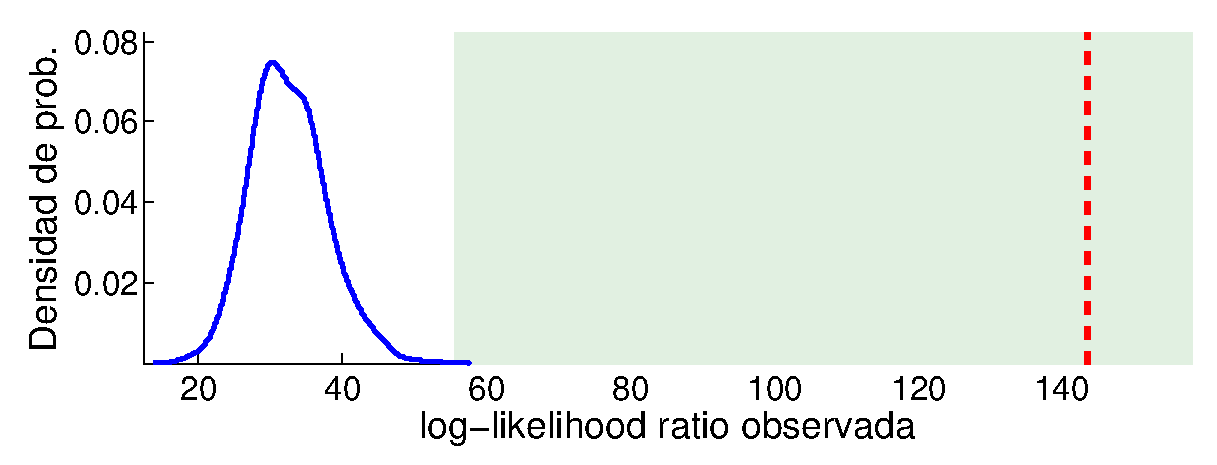
\includegraphics[width=1\linewidth]{gfx/chap6/lear3boot2}
      \caption{}
      \label{fig:seq3_boot2}
    \end{subfigure}
  }
  \centerline  
  { \begin{subfigure}[b]{0.7\textwidth}
      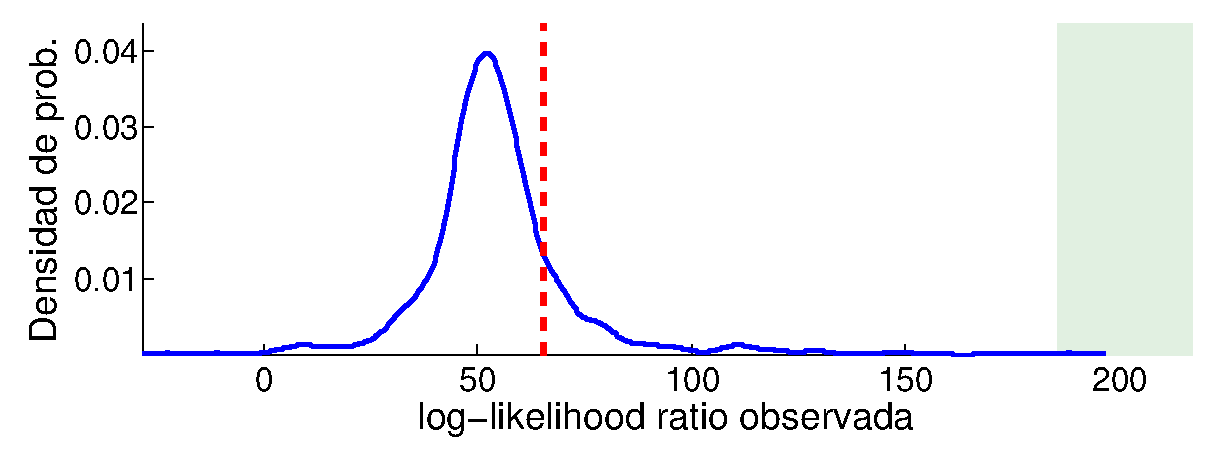
\includegraphics[width=1\linewidth]{gfx/chap6/lear3boot3}
      \caption{}
      \label{fig:seq3_boot3}
    \end{subfigure}
    \hspace{0.5cm}
    \begin{subfigure}[b]{0.7\textwidth}
      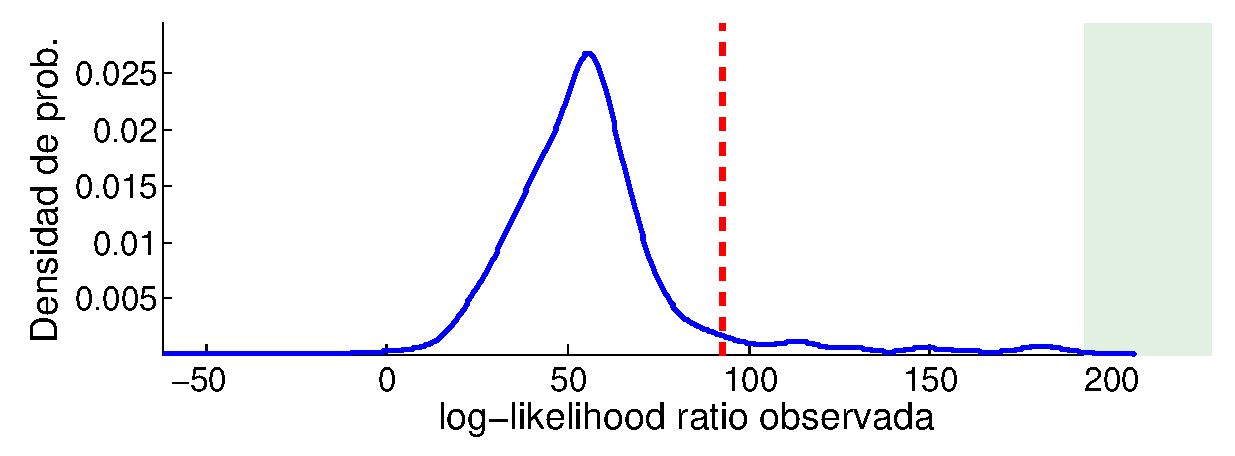
\includegraphics[width=1\linewidth]{gfx/chap6/lear3boot4}
      \caption{}
      \label{fig:seq3_boot4}
    \end{subfigure}
  }
  \caption[Secuencia 3: Pruebas de hipótesis usando bootstrap]{En la \autoref{fig:seq3_boot1} se muestra la prueba de hipótesis realizada para comparar el modelo $n_4$ contra $n_5$. Como se observa, se rechaza la hipótesis de que el modelo correcto sea $n_4$. En la \autoref{fig:seq3_boot2} se hace la prueba del modelo $n_5$ contra $n_6$, y de la misma manera, se rechaza la hipótesis de que el modelo correcto sea $n_5$. Se sigue con la prueba de hipótesis del modelo $n_6$ contra $n_7$ en la \autoref{fig:seq3_boot3}, y en este caso el valor observado no cae dentro de la región de rechazo, por lo que no podemos rechazar que el modelo $n_6$ sea el correcto. Por último en la \autoref{fig:seq3_boot4}, se hace la prueba del modelo $n_7$ contra el modelo $n_8$, y se vuelve a rechazar la hipótesis nula.}  
  \label{fig:seq3_boot}
\end{figure}

En caso de que después de utilizar BIC se presente ambigüedad para determinar un modelo ganador, o ya sea para realizar un análisis más exhaustivo, se puede propone hacer una prueba de hipótesis para determinar cuál modelo se ajusta mejor a los datos.

A diferencia de la primer etapa, en la que se usa BIC como criterio para  seleccionar el mejor modelo de un conjunto no definido de modelos con diferentes parámetros, la intención de hacer pruebas de hipótesis es determinar en un pequeño conjunto de probables modelos, cuál es mejor, y qué tan bueno es un modelo respecto a otro.

Al plantear la prueba de hipótesis se harán una gran cantidad de simulaciones para ver qué tan bien se ajusta cada modelo a los datos originales, por lo que este proceso es computacionalmente intensivo y sólo se recomienda hacerlo para evitar la ambigüedad entre un par de modelos.

...

Por último, ya con el modelo seleccionado, se procede a calcular el error relativo de predicción que se obtuvo, comparando con el ground truth que se dispone para esa secuencia, con lo que se obtiene: 

...

\begin{figure}[tp]
  \centerline
  {\begin{subfigure}[b]{1.3\textwidth}
      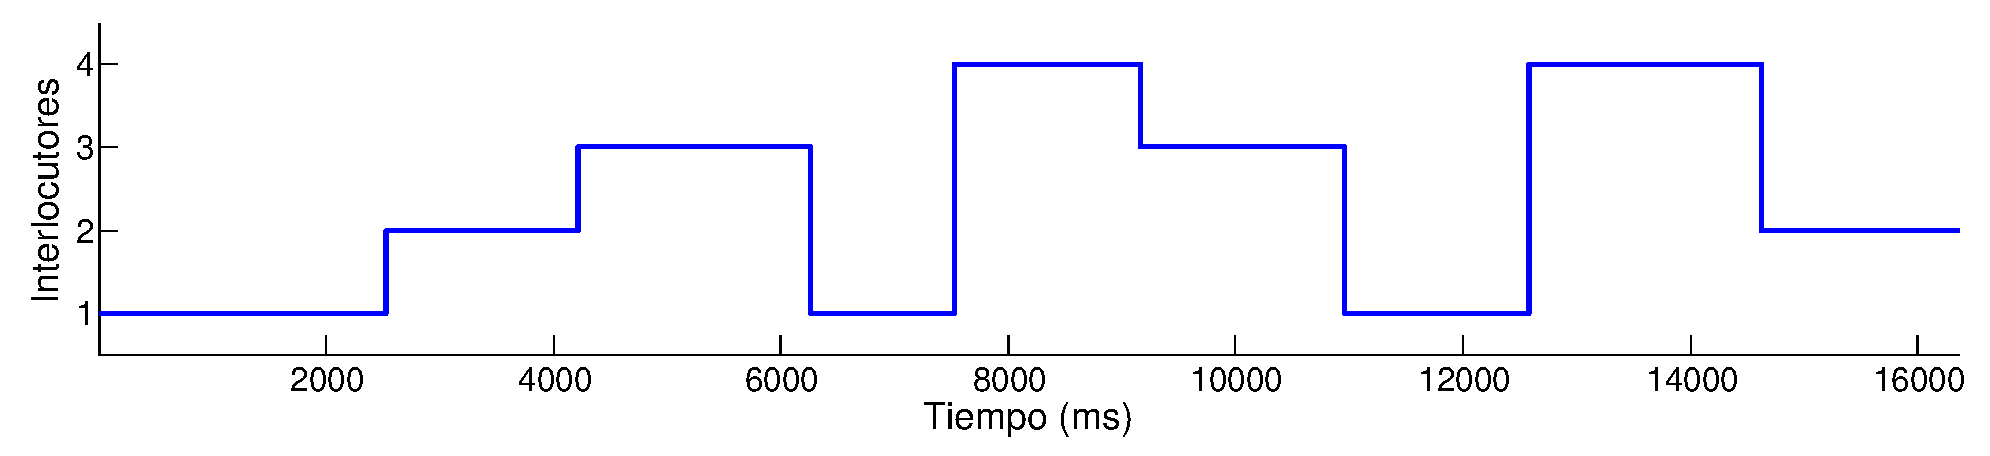
\includegraphics[width=1\linewidth]{gfx/chap6/lear3s_3_1}
      \caption{}
      \label{fig:seq3_seq1}
    \end{subfigure}
  } 
  \centerline
  {\begin{subfigure}[b]{1.3\textwidth}
      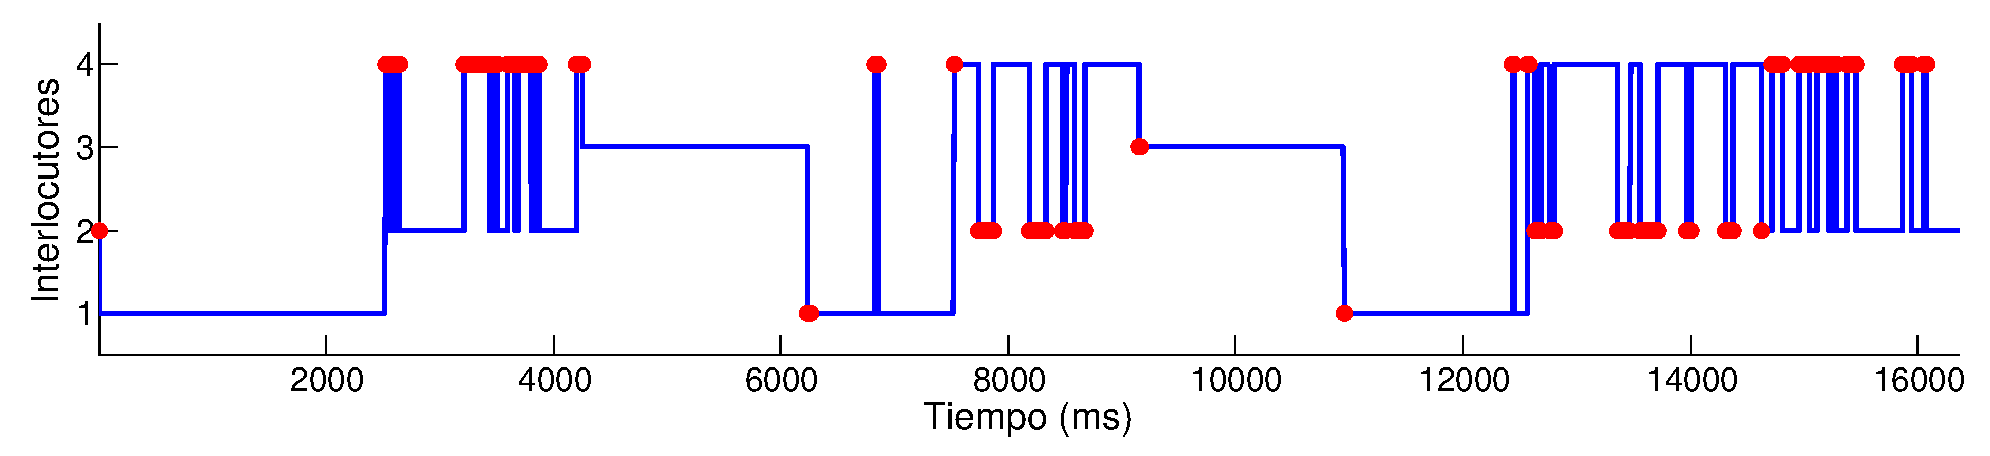
\includegraphics[width=1\linewidth]{gfx/chap6/lear3s_3_2}
      \caption{}
      \label{fig:seq3_seq2}
    \end{subfigure}
  }
  \caption[Secuencia 3: Secuencia recuperada]{En \autoref{fig:seq3_seq1} se muestra la secuencia original de la \autoref{ssub:lear}. En comparación, en \autoref{fig:seq3_seq2} se muestra la secuencia recuperada del modelo ganador y se marcan en rojo los errores cometidos respecto a la primera secuencia. }
  \label{fig:prb3_seq}
\end{figure}

Más a detalle, en la \autoref{fig:prb3_seq} se observa en azul el orden en el que participan los interlocutores de acuerdo a la secuencia recuperada. En rojo se marcan tanto los falsos positivos como los falsos negativos, de acuerdo al ground truth. Hay que notar que cuando el número de estados para un modelo no es el correcto, entonces inminentemente el número de errores en la secuencia obtenida será mayor, pues al menos todas las intervenciones de un hablante no podrán ser emparejadas o serán asignadas a alguien más.

Se observa también que la mayoría de las veces, en la secuencia recuperada se encuentran algunos brincos entre personas, pero en esencia la estructura y el orden en que hablan los interlocutores es el correcto.
 

%%%%%%%%%%%%%%%%%%%%%%%%%%%%%%%%%%%%%%%%%%%%%%%%%%%%%%%%%%%%%%% 

\subsection[Secuencia 4]{Secuencia 4: Manuel Acuña}
\label{ssub:nocturno}

  Para la cuarta secuencia se utilizaron algunos poemas del escritor Manuel Acuña, alternando 6 voces diferentes en español. La secuencia de audio original tiene una duración de 10:41 min.

Para la etapa de agrupación de los vectores MFCC con k-means++ se usaron 140 centros iniciales, mientras que el banco de filtros fue el mismo que en la secuencia anterior.

\begin{figure}[tp]
  \centerline{  
    \hspace{1.2cm}
    \parbox[c]{0.38\textwidth}{\centering Modelo generador}
    \parbox[c]{0.38\textwidth}{\centering Modelo $n_2$}
    \parbox[c]{0.38\textwidth}{\centering Modelo $n_3$}
    \parbox[c]{0.38\textwidth}{\centering Modelo $n_4$}
  }
  \vspace{0.5cm}
  \foreach \row in {1, ..., 2}{%  
    \centerline{%
      \parbox[c]{1cm}{
        \vspace{-0.5cm}
        \myheader{\row}
      }
      %\gdef \widthimg {0.35}
      \foreach \col in {1, ..., 4}{%
        \pgfmathparse{\col == 4 && \row == 2? 1:0}
        \ifthenelse{\pgfmathresult=1}{
          \gdef \widthimg {0.39}
        }{
          \gdef \widthimg {0.35}
        }
        \begin{subfigure}[c]{\widthimg \textwidth}          
          \def \imgfile {gfx/chap6/noct1p_\col_\row}
          \IfFileExists{\imgfile.eps}{
            \includegraphics[width=1\textwidth]{\imgfile}
            \label{fig:seq4p_\col_\row}
          }{
            \hspace{1\textwidth}
          }
        \end{subfigure}
        %\hspace{-0.005\textwidth}
      }
    }
  }
\caption[Secuencia 4: Parámetros estimados (1)]{Por columnas, se muestran los parámetros obtenidos para varios modelos propuestos. La primer columna corresponde a los parámetros verdaderos.
En la primer fila \textup{(a)} se muestran las probabilidades a priori de que cada uno de los interlocutores empiecen la conversación. En la segunda fila \textup{(b)} se muestra en falso color la matriz de transición entre interlocutores para cada uno de los modelos mostrados.}
\label{fig:seq4p}
\end{figure}

En las \autoref{fig:seq4p} y \autoref{fig:seq4q} se muestran los parámetros estimados para los diferentes modelos que se propusieron. La primer columna corresponde a los parámetros verdaderos, mientras que las demás columnas son los parámetros obtenidos para diferentes modelos estimados. 

En la primer fila de la \autoref{fig:seq4p} se muestran las probabilidades a priori de que cada uno de los interlocutores empiecen el diálogo. En la segunda fila se muestra en falso color la matriz de transición para cada uno de los modelos. Esta matriz representa la probabilidad de cambio entre las personas que participan en la conversación.

Se observa como en general para todos los modelos propuestos la matriz de transición que se recupera tiene una estructura diagonal, puesto que en este tipo de problemas, una persona suele hablar durante un periodo considerablemente largo, para que luego otra persona empiece a hablar.

\begin{figure}[t!]
  \centerline{
    \hspace{1.2cm}
    \parbox[c]{0.35\textwidth}{\centering Modelo generador}
    \parbox[c]{0.35\textwidth}{\centering Modelo $n_2$}
    \parbox[c]{0.35\textwidth}{\centering Modelo $n_3$}
    \parbox[c]{0.35\textwidth}{\centering Modelo $n_4$}
  }
  \vspace{0.5cm}
  \foreach \row in {3, ..., 6}{%  
    \centerline{
      \parbox[c]{1cm}{
        \vspace{-0.3cm}
        \myheader{\row}
      }
      \foreach \col in {1, ..., 4}{%
        \begin{subfigure}[c]{0.35\textwidth}  
          \def \imgfile {gfx/chap6/noct1p_\col_\row}
          \IfFileExists{\imgfile.eps}{
            \includegraphics[width=1\textwidth]{\imgfile}
            %\caption{}
            \label{fig:seq4p_\col_\row}
          }{
            \hspace{1\textwidth}
          }
        \end{subfigure}
      }
    }
  }
\caption[Secuencia 4: Parámetros estimados (2)]{Por columnas, se muestran las probabilidades de emisión para cada uno de los interlocutores de acuerdo al modelo. Cada fila representa las probabilidad de emisión de las palabras en el diccionario. La fila \textup{(c)} para la primer persona, la fila \textup{(d)} para la segunda persona y así de forma consecutiva, de acuerdo al número de personas que contempla cada modelo propuesto.}
\label{fig:seq4q}
\end{figure}

En la \autoref{fig:seq4q} se muestran las probabilidades de emisión para cada uno de los participantes, de acuerdo a las palabras en las que se ha discretizado la conversación. Idealmente, cada interlocutor tiene asignadas con mayor probabilidad un cierto conjunto de palabras del diccionario, lo que hace que la identificación de las personas sea mucho más fácil de realizar.

Para la selección del modelo y siguiendo la metodología propuesta, primero se efectúa una inspección por medio de BIC regularizado para encontrar cuál o cuáles son los modelos más probables.

\begin{figure}[t!]
  \centerline{
  \begin{subfigure}[b]{1.1\textwidth}
   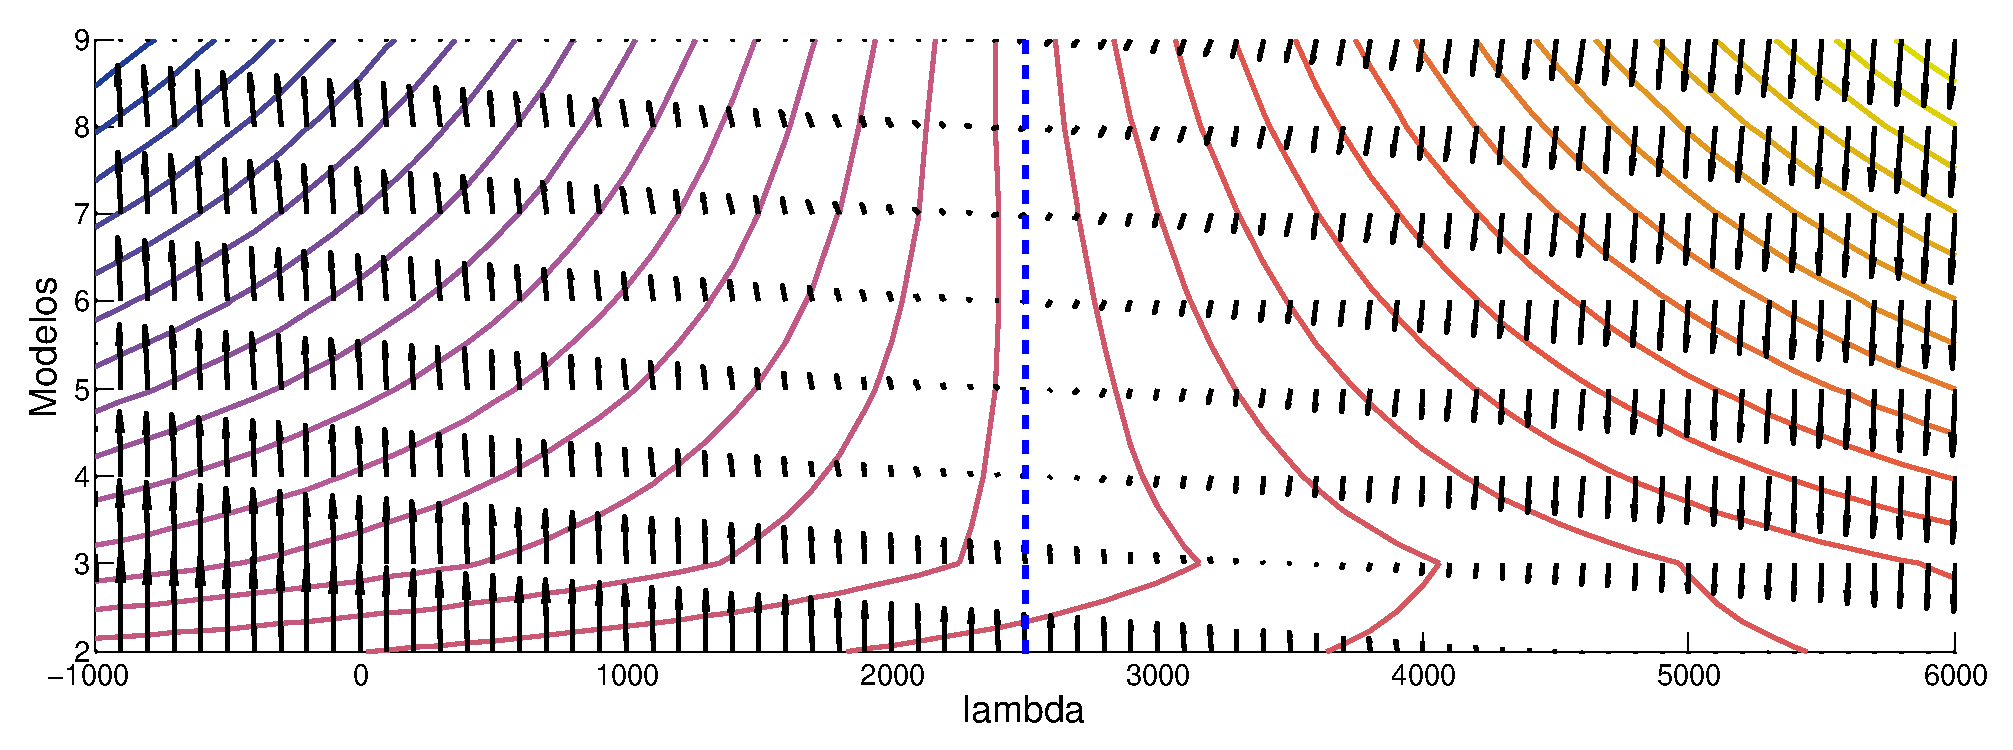
\includegraphics[width=1\textwidth]{gfx/chap6/noct1bic2}
   \caption{}
   \label{fig:seq4_bic2}
  \end{subfigure}  
  }  
  \centerline{
  \begin{subfigure}[b]{0.55\textwidth}
    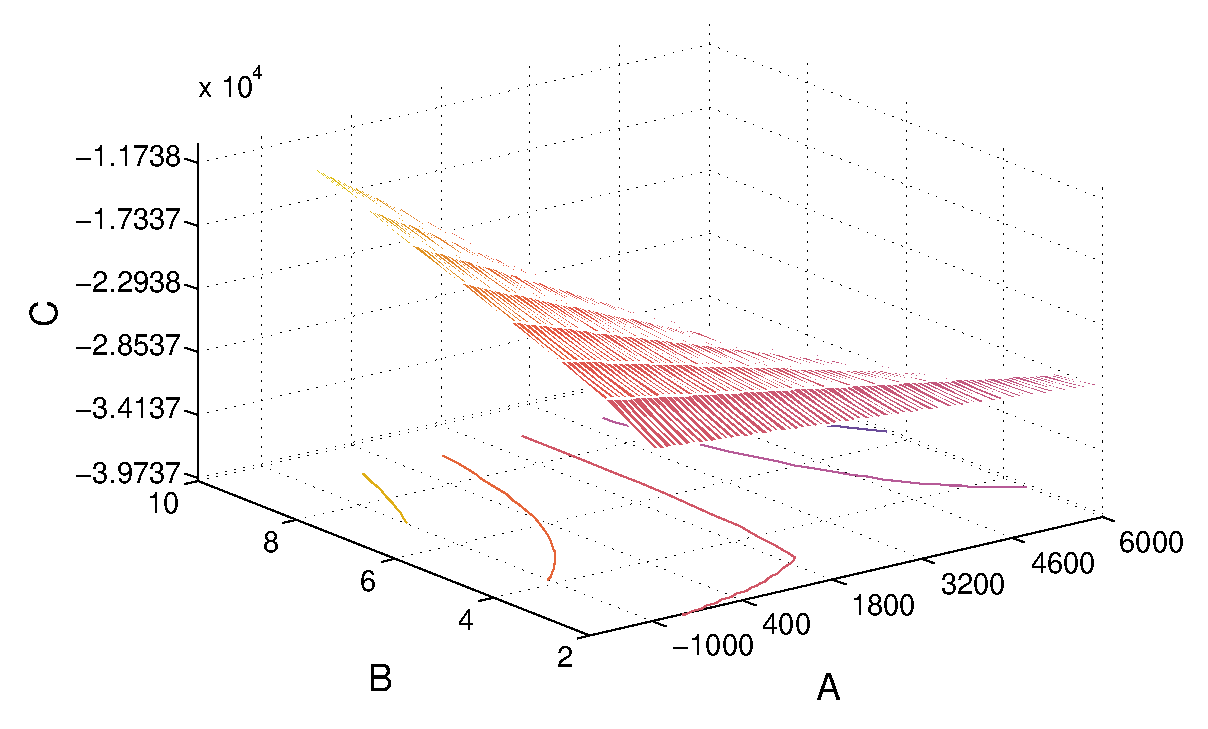
\includegraphics[width=\textwidth]{gfx/chap6/noct1bic1} 
    \caption{}
    \label{fig:seq4_bic1}
  \end{subfigure}  
  \begin{subfigure}[b]{0.55\textwidth}
    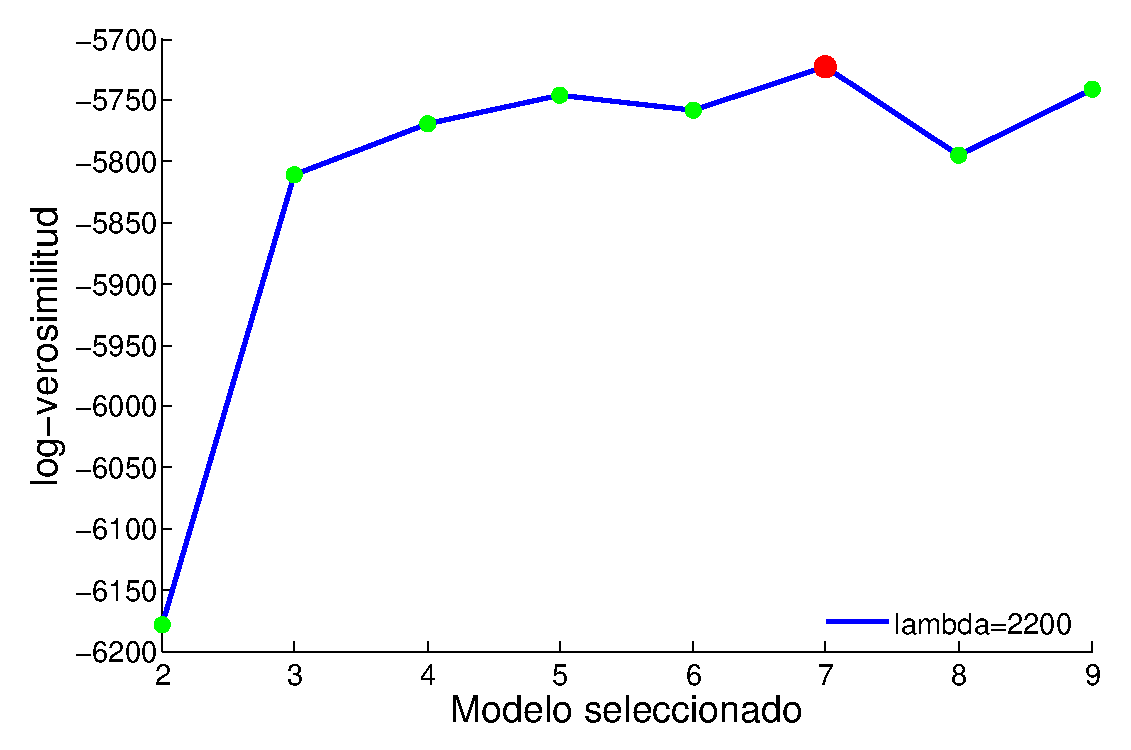
\includegraphics[width=\textwidth]{gfx/chap6/lear3bic3} 
    \caption{}
    \label{fig:seq4_bic3}
  \end{subfigure}
  }
  \caption[Secuencia 4: Pruebas BIC]{En la \autoref{fig:seq4_bic2}, se muestra las curvas de nivel de la superficie al variar el valor de lambda para evaluar BIC, así como la dirección del gradiente en la misma. En la \autoref{fig:seq4_bic1} se muestra una perspectiva general de superficie en \autoref{fig:seq4_bic2}. En la \autoref{fig:seq4_bic3} se muestra el valor seleccionado para lambda de acuerdo al análisis de sensibilidad realizado en la superficie anterior.}
  \label{fig:seq4_bic}
\end{figure}

En la \autoref{fig:seq4_bic1} se muestra la superficie generada al variar el valor de $\lambda$ para diferentes curvas de selección BIC. Se observa cómo al principio $\lambda$ es muy pequeño, y entonces el término de penalización no funciona por lo que se prefieren los modelos más complejos y sobre ajustados. Por otro lado, cuando $\lambda$ es muy grande, la penalización no permite mas que escoger los modelos más simples.

Haciendo un análisis de sensibilidad se puede determinar cuál es el parámetro $\lambda$ adecuado que penaliza de buena forma la log-verosimilitud.

En la \autoref{fig:seq4_bic2} se muestran las curvas de nivel de la figura anterior, además de la dirección del gradiente de la misma. Así mismo, en falso color se resaltan las zonas en las que el gradiente es menor. 

Lo que nos interesa encontrar en la superficie, es el valor de $\lambda$ que representa el punto de inflexión entre la selección de modelos demasiado complejos y modelos más simples. Para esto, se busca la zona en la que el gradiente sea lo más cercano a cero, pues implicaría que es un punto crítico.

Debido a la escala y a la forma en la que se calculó el gradiente, aunque para algunos valores cercanos de $\lambda$ no haya mucha variación en esa dirección; si BIC está penalizando mal, entonces sí habrá gran variación para los diferentes modelos. Es por esto, que sólo en la zona en que la penalización sea del mismo orden de magnitud que la verosimilitud la variación en la curva BIC con el $\lambda$ adecuado no será tan grande como en otras zonas.

Por último, se muestra en \autoref{fig:seq4_bic3} la curva BIC con el valor de $\lambda$ encontrado a partir del análisis de sensibilidad realizado en la \autoref{fig:seq4_bic2}. El o los modelos que tengan un mayor valor BIC serán los que se seleccionarán como modelos ganadores.

\begin{figure}[t!]
  \centerline  
  { \begin{subfigure}[b]{0.7\textwidth}
      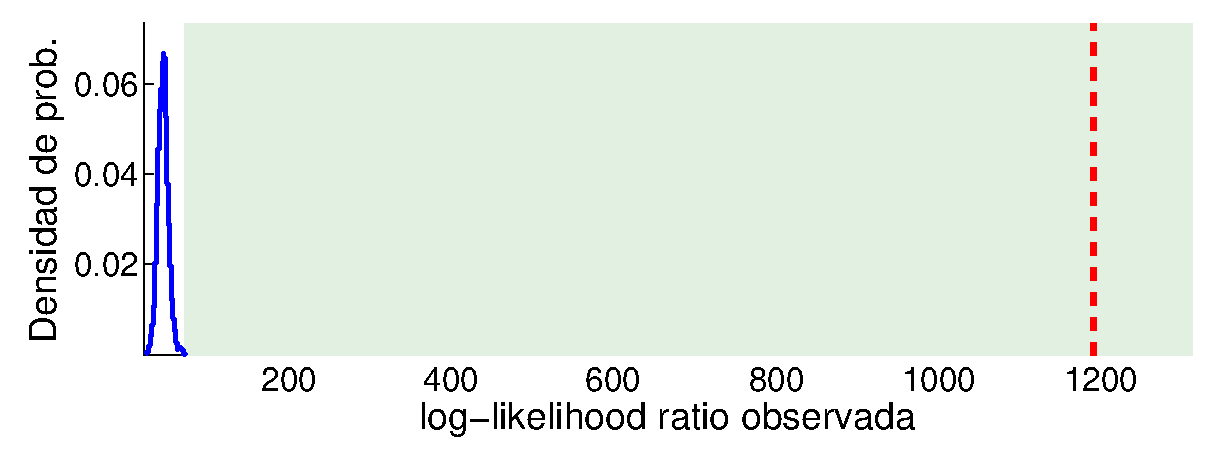
\includegraphics[width=1\linewidth]{gfx/chap6/noct1boot1}
      \caption{}
      \label{fig:seq4_boot1}
    \end{subfigure}
    \hspace{0.5cm}
    \begin{subfigure}[b]{0.7\textwidth}
      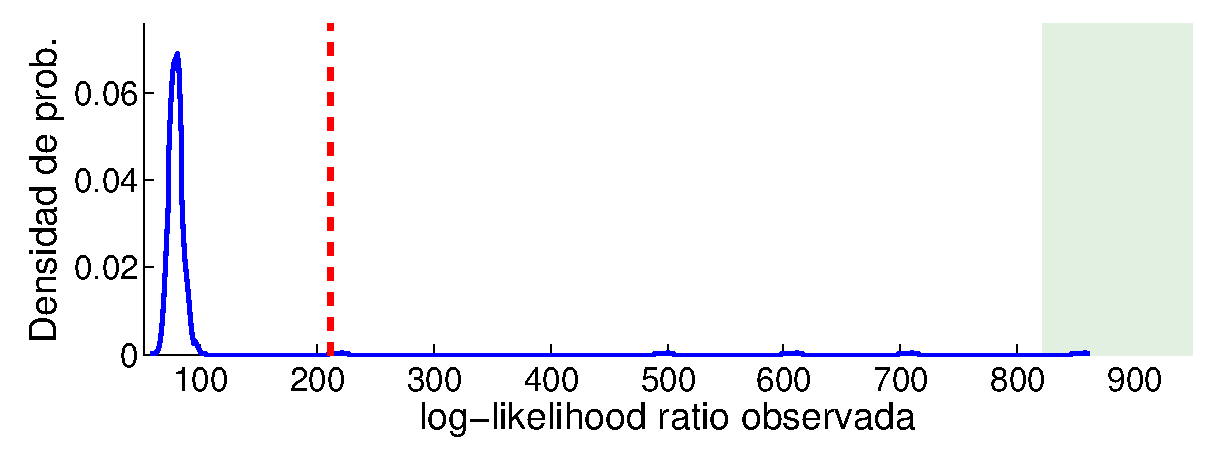
\includegraphics[width=1\linewidth]{gfx/chap6/noct1boot2}
      \caption{}
      \label{fig:seq4_boot2}
    \end{subfigure}
  }
  \centerline  
  { \begin{subfigure}[b]{0.7\textwidth}
      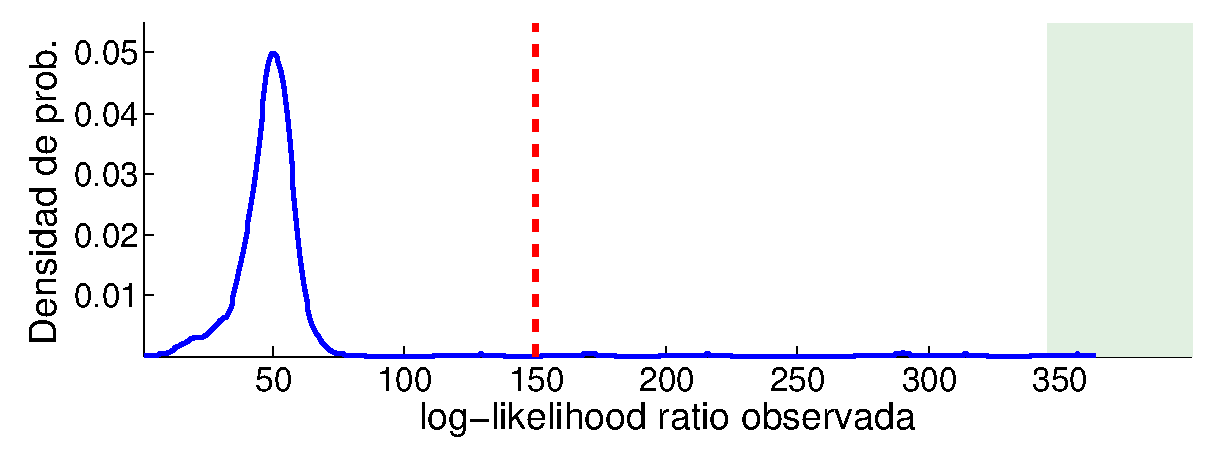
\includegraphics[width=1\linewidth]{gfx/chap6/noct1boot3}
      \caption{}
      \label{fig:seq4_boot3}
    \end{subfigure}
    \hspace{0.5cm}
    \begin{subfigure}[b]{0.7\textwidth}
      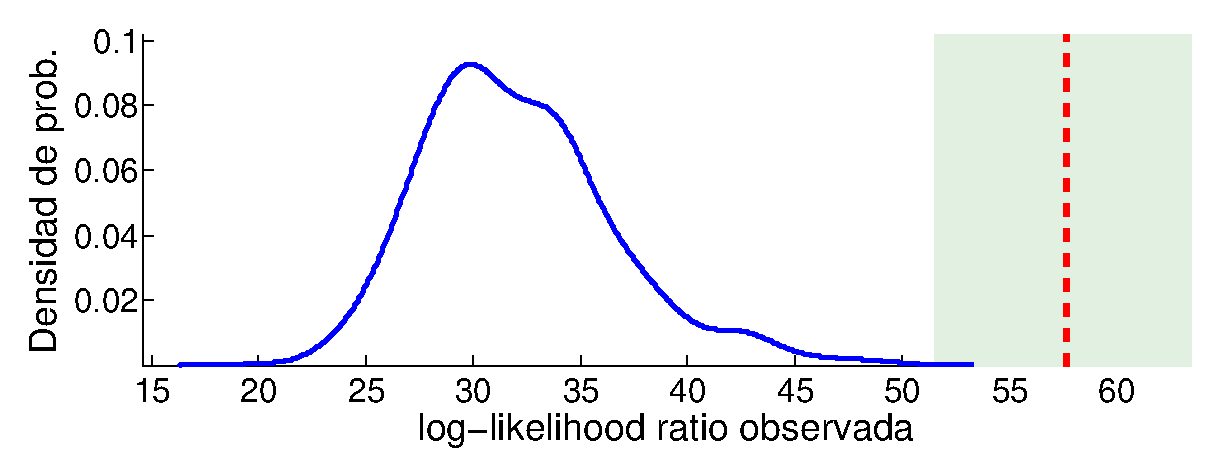
\includegraphics[width=1\linewidth]{gfx/chap6/noct1boot4}
      \caption{}
      \label{fig:seq4_boot4}
    \end{subfigure}
  }
  \caption[Secuencia 4: Pruebas de hipótesis usando bootstrap]{En la \autoref{fig:seq4_boot1} se muestra la prueba de hipótesis realizada para comparar el modelo $n_4$ contra $n_5$. Como se observa, se rechaza la hipótesis de que el modelo correcto sea $n_4$. En la \autoref{fig:seq4_boot2} se hace la prueba del modelo $n_5$ contra $n_6$, y de la misma manera, se rechaza la hipótesis de que el modelo correcto sea $n_5$. Se sigue con la prueba de hipótesis del modelo $n_6$ contra $n_7$ en la \autoref{fig:seq4_boot3}, y en este caso el valor observado no cae dentro de la región de rechazo, por lo que no podemos rechazar que el modelo $n_6$ sea el correcto. Por último en la \autoref{fig:seq4_boot4}, se hace la prueba del modelo $n_7$ contra el modelo $n_8$, y se vuelve a rechazar la hipótesis nula.}  
  \label{fig:seq4_boot}
\end{figure}

En caso de que después de utilizar BIC se presente ambigüedad para determinar un modelo ganador, o ya sea para realizar un análisis más exhaustivo, se puede propone hacer una prueba de hipótesis para determinar cuál modelo se ajusta mejor a los datos.

A diferencia de la primer etapa, en la que se usa BIC como criterio para  seleccionar el mejor modelo de un conjunto no definido de modelos con diferentes parámetros, la intención de hacer pruebas de hipótesis es determinar en un pequeño conjunto de probables modelos, cuál es mejor, y qué tan bueno es un modelo respecto a otro.

Al plantear la prueba de hipótesis se harán una gran cantidad de simulaciones para ver qué tan bien se ajusta cada modelo a los datos originales, por lo que este proceso es computacionalmente intensivo y sólo se recomienda hacerlo para evitar la ambigüedad entre un par de modelos.

...

Por último, ya con el modelo seleccionado, se procede a calcular el error relativo de predicción que se obtuvo, comparando con el ground truth que se dispone para esa secuencia, con lo que se obtiene: 

...

\begin{figure}[tp]
  \centerline
  {\begin{subfigure}[b]{1.3\textwidth}
      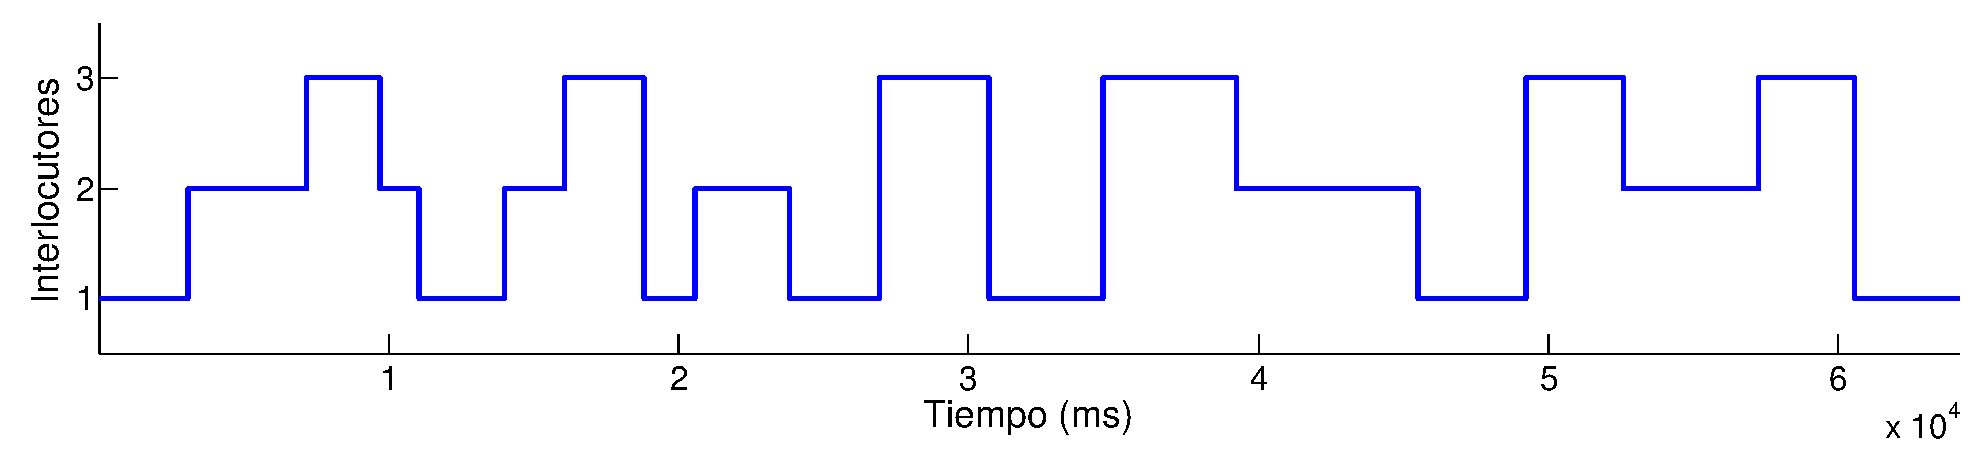
\includegraphics[width=1\linewidth]{gfx/chap6/noct1s_3_1}
      \caption{}
      \label{fig:seq4_seq1}
    \end{subfigure}
  } 
  \centerline
  {\begin{subfigure}[b]{1.3\textwidth}
      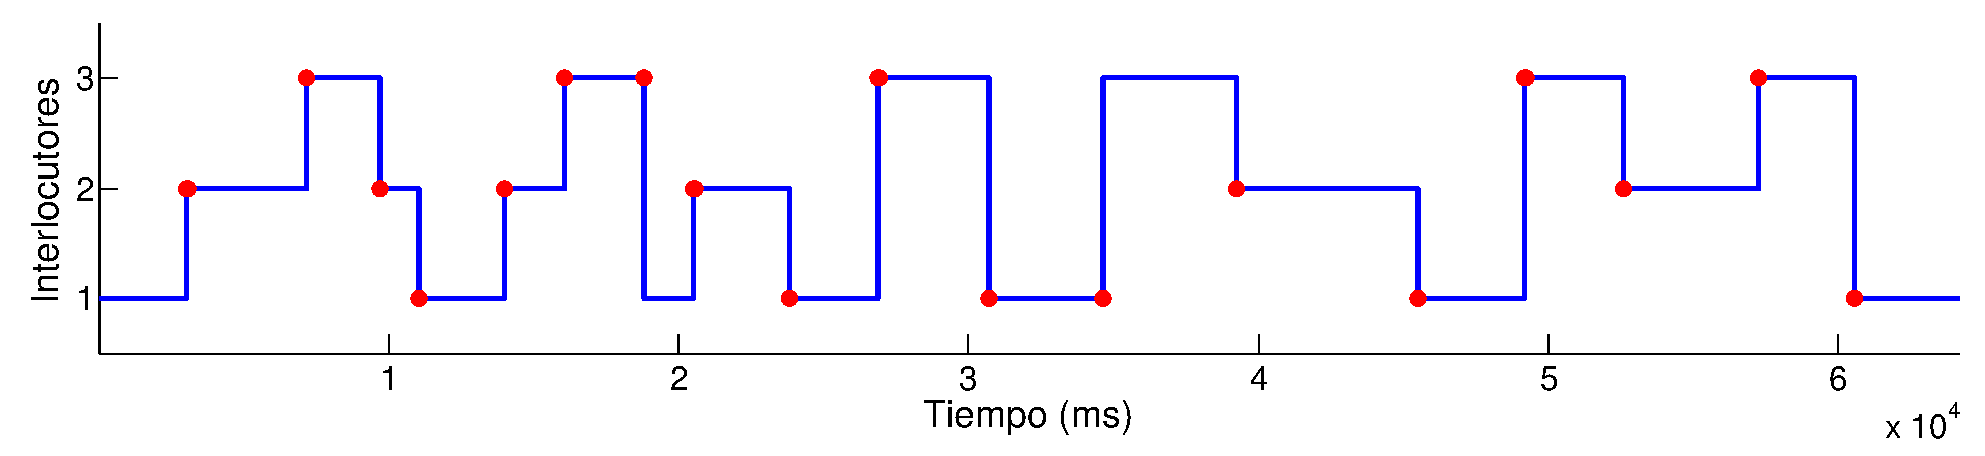
\includegraphics[width=1\linewidth]{gfx/chap6/noct1s_3_2}
      \caption{}
      \label{fig:seq4_seq2}
    \end{subfigure}
  }
  \caption[Secuencia 4: Secuencia recuperada]{En \autoref{fig:seq4_seq1} se muestra la secuencia original de la \autoref{ssub:nocturno}. En comparación, en \autoref{fig:seq4_seq2} se muestra la secuencia recuperada del modelo ganador y se marcan en rojo los errores cometidos respecto a la primera secuencia. }
  \label{fig:prb4_seq}
\end{figure}

Más a detalle, en la \autoref{fig:prb4_seq} se observa en azul el orden en el que participan los interlocutores de acuerdo a la secuencia recuperada. En rojo se marcan tanto los falsos positivos como los falsos negativos, de acuerdo al ground truth. Hay que notar que cuando el número de estados para un modelo no es el correcto, entonces inminentemente el número de errores en la secuencia obtenida será mayor, pues al menos todas las intervenciones de un hablante no podrán ser emparejadas o serán asignadas a alguien más.

Se observa también que la mayoría de las veces, en la secuencia recuperada se encuentran algunos brincos entre personas, pero en esencia la estructura y el orden en que hablan los interlocutores es el correcto.
 

%%%%%%%%%%%%%%%%%%%%%%%%%%%%%%%%%%%%%%%%%%%%%%%%%%%%%%%%%%%%%%% 

\subsection[Secuencia 5]{Secuencia 5: Calderón de la Barca}
\label{ssub:calderon}

  En esta quinta secuencia se trabajó con varios fragmentos del poema 'La vida es sueño' del escritor Pedro Calderón de la Barca, usándose 3 diferentes voces en español. La secuencia de audio original es de 11:18 min.

Para la etapa de agrupación de los vectores MFCC con k-means++ se usaron 160 centros iniciales, mientras que el banco de filtros fue el usado en las secuencias anteriores.

\begin{figure}[bht]
  \centerline{  
    \hspace{1.2cm}
    \parbox[c]{0.38\textwidth}{\centering Modelo generador}
    \parbox[c]{0.38\textwidth}{\centering Modelo $n_2$}
    \parbox[c]{0.38\textwidth}{\centering Modelo $n_3$}
    \parbox[c]{0.38\textwidth}{\centering Modelo $n_4$}
  }
  \vspace{0.5cm}
  \foreach \row in {1, ..., 2}{%  
    \centerline{%
      \parbox[c]{1cm}{
        \vspace{-0.5cm}
        \myheader{\row}
      }
      %\gdef \widthimg {0.35}
      \foreach \col in {1, ..., 4}{%
        \pgfmathparse{\col == 4 && \row == 2? 1:0}
        \ifthenelse{\pgfmathresult=1}{
          \gdef \widthimg {0.39}
        }{
          \gdef \widthimg {0.35}
        }
        \begin{subfigure}[c]{\widthimg \textwidth}          
          \def \imgfile {gfx/chap6/calderon1p_\col_\row}
          \IfFileExists{\imgfile.eps}{
            \includegraphics[width=1\textwidth]{\imgfile}
            \label{fig:seq5p_\col_\row}
          }{
            \hspace{1\textwidth}
          }
        \end{subfigure}
        %\hspace{-0.005\textwidth}
      }
    }
  }
\caption[Secuencia 5: Parámetros estimados (1)]{Por columnas, se muestran los parámetros obtenidos para varios modelos propuestos. La primer columna corresponde a los parámetros verdaderos.
En la primer fila \textup{(a)} se muestran las probabilidades a priori de que cada uno de los interlocutores empiecen la conversación. En la segunda fila \textup{(b)} se muestra en falso color la matriz de transición entre interlocutores para cada uno de los modelos mostrados.}
\label{fig:seq5p}
\end{figure}

En las \autoref{fig:seq5p} y \autoref{fig:seq5q} se muestran los parámetros estimados para los diferentes modelos que se propusieron. La primer columna corresponde a los parámetros verdaderos, mientras que las demás columnas son los parámetros obtenidos para diferentes modelos estimados. 

En la primer fila de la \autoref{fig:seq5p} se muestran las probabilidades a priori de que cada uno de los interlocutores empiecen el diálogo. En la segunda fila se muestra en falso color la matriz de transición para cada uno de los modelos. Esta matriz representa la probabilidad de cambio entre las personas que participan en la conversación.

Se observa como en general para todos los modelos propuestos la matriz de transición que se recupera tiene una estructura diagonal, puesto que en este tipo de problemas, una persona suele hablar durante un periodo considerablemente largo, para que luego otra persona empiece a hablar.

\begin{figure}[t!]
  \centerline{
    \hspace{1.2cm}
    \parbox[c]{0.35\textwidth}{\centering Modelo generador}
    \parbox[c]{0.35\textwidth}{\centering Modelo $n_2$}
    \parbox[c]{0.35\textwidth}{\centering Modelo $n_3$}
    \parbox[c]{0.35\textwidth}{\centering Modelo $n_4$}
  }
  \vspace{0.5cm}
  \foreach \row in {3, ..., 6}{%  
    \centerline{
      \parbox[c]{1cm}{
        \vspace{-0.3cm}
        \myheader{\row}
      }
      \foreach \col in {1, ..., 4}{%
        \begin{subfigure}[c]{0.35\textwidth}  
          \def \imgfile {gfx/chap6/calderon1p_\col_\row}
          \IfFileExists{\imgfile.eps}{
            \includegraphics[width=1\textwidth]{\imgfile}
            %\caption{}
            \label{fig:seq5p_\col_\row}
          }{
            \hspace{1\textwidth}
          }
        \end{subfigure}
      }
    }
  }
\caption[Secuencia 5: Parámetros estimados (2)]{Por columnas, se muestran las probabilidades de emisión para cada uno de los interlocutores de acuerdo al modelo. Cada fila representa las probabilidad de emisión de las palabras en el diccionario. La fila \textup{(c)} para la primer persona, la fila \textup{(d)} para la segunda persona y así de forma consecutiva, de acuerdo al número de personas que contempla cada modelo propuesto.}
\label{fig:seq5q}
\end{figure}

En la \autoref{fig:seq5q} se muestran las probabilidades de emisión para cada uno de los participantes, de acuerdo a las palabras en las que se ha discretizado la conversación. Idealmente, cada interlocutor tiene asignadas con mayor probabilidad un cierto conjunto de palabras del diccionario, lo que hace que la identificación de las personas sea mucho más fácil de realizar.

Para la selección del modelo y siguiendo la metodología propuesta, primero se efectúa una inspección por medio de BIC regularizado para encontrar cuál o cuáles son los modelos más probables.

\begin{figure}[t!]
  \centerline{
  \begin{subfigure}[b]{1.1\textwidth}
   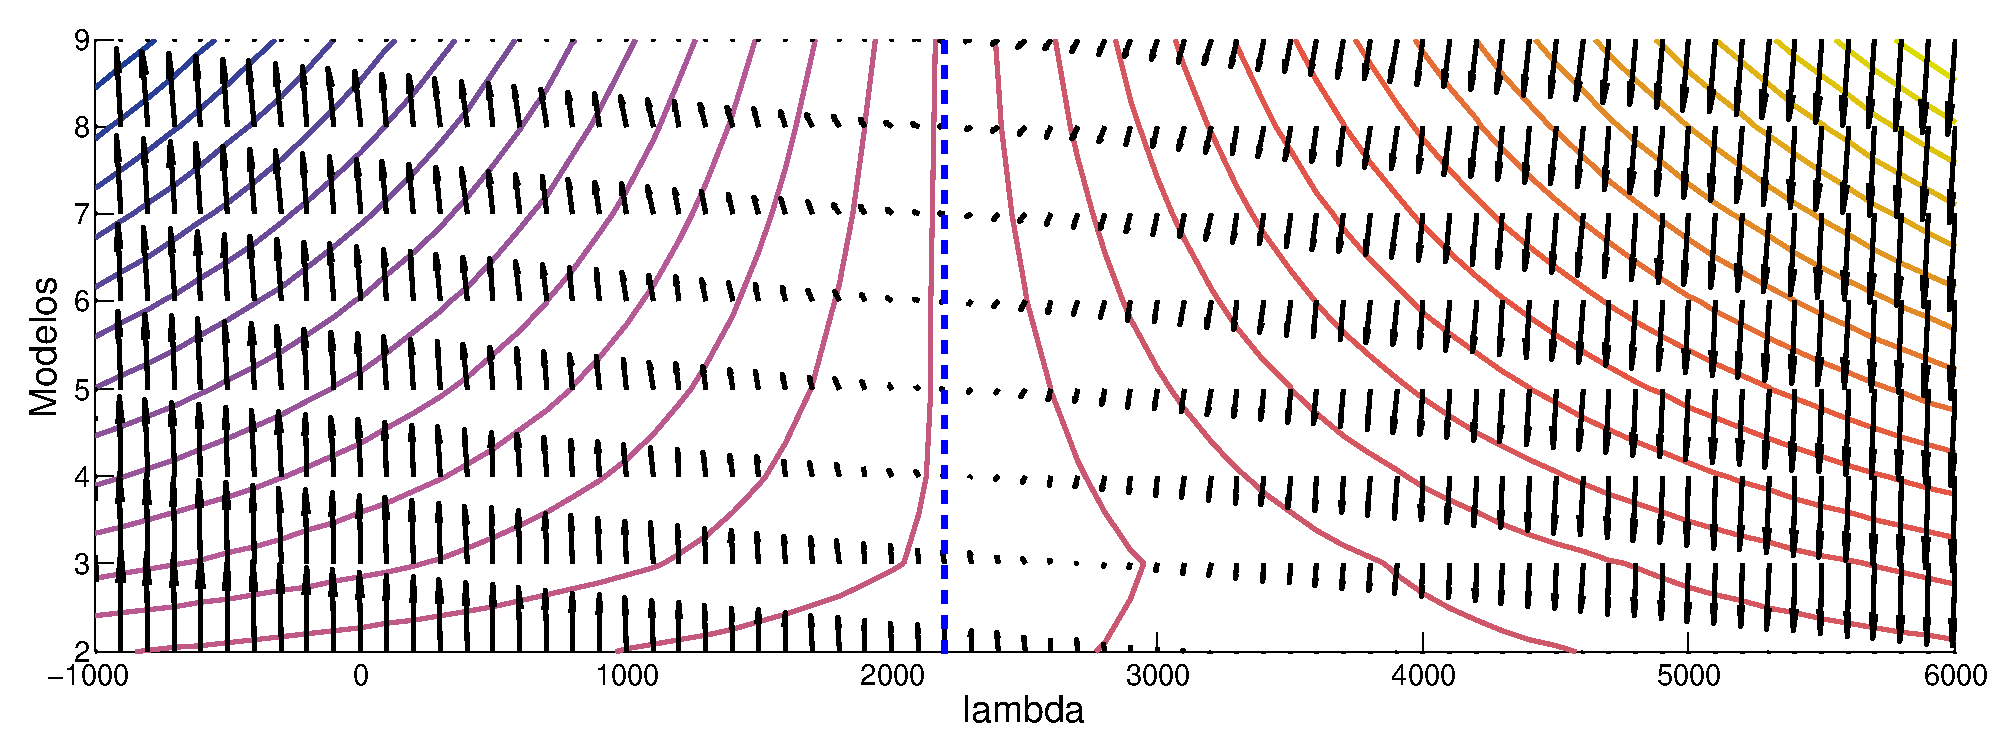
\includegraphics[width=1\textwidth]{gfx/chap6/calderon1bic2}
   \caption{}
   \label{fig:seq5_bic2}
  \end{subfigure}  
  }  
  \centerline{
  \begin{subfigure}[b]{0.55\textwidth}
    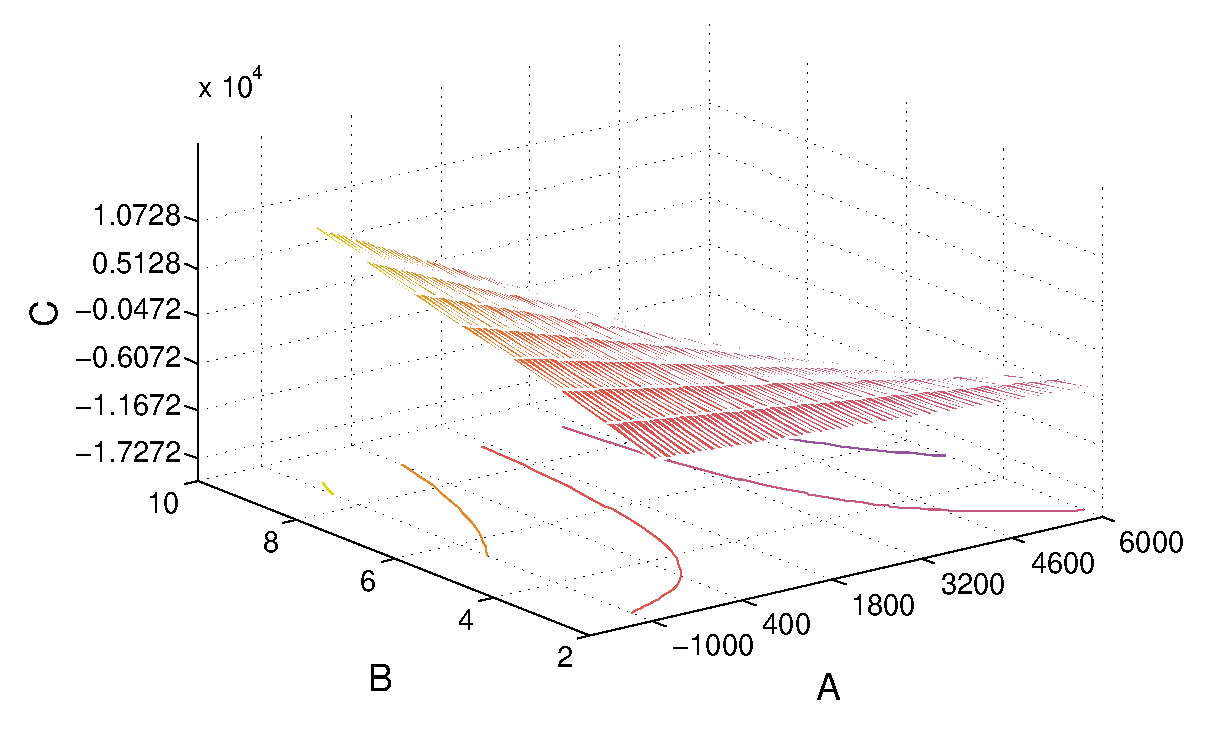
\includegraphics[width=\textwidth]{gfx/chap6/calderon1bic1} 
    \caption{}
    \label{fig:seq5_bic1}
  \end{subfigure}  
  \begin{subfigure}[b]{0.55\textwidth}
    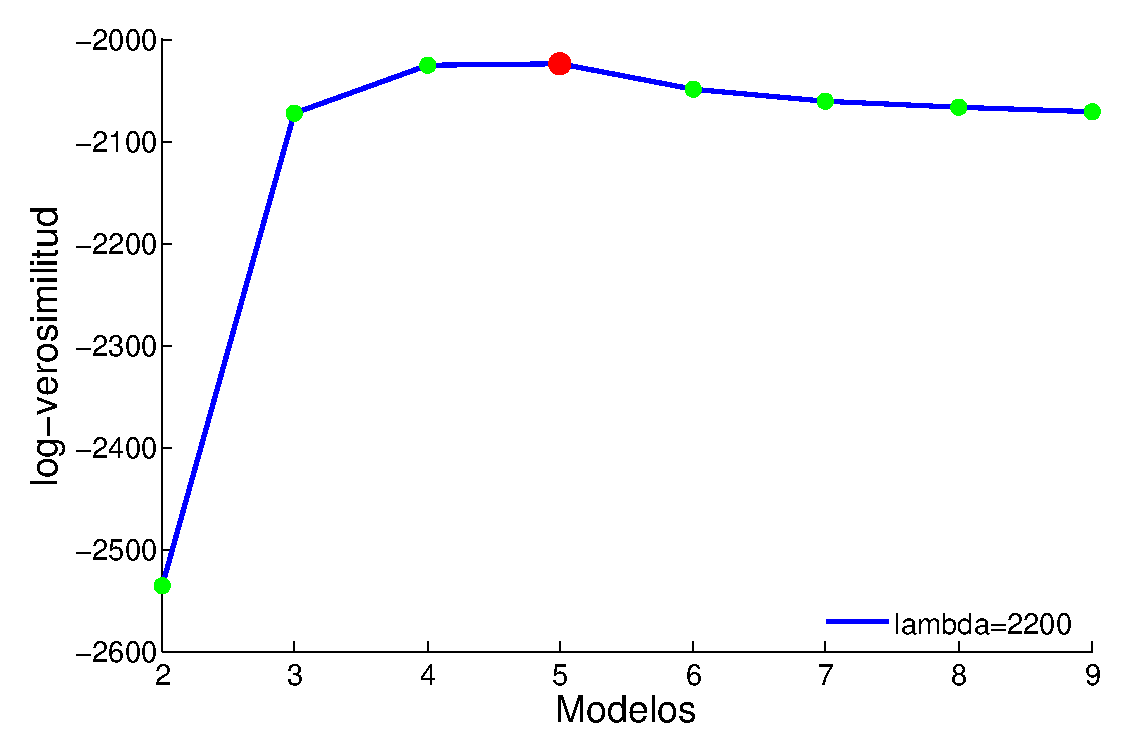
\includegraphics[width=\textwidth]{gfx/chap6/calderon1bic3} 
    \caption{}
    \label{fig:seq5_bic3}
  \end{subfigure}
  }
  \caption[Secuencia 5: Pruebas BIC]{En la \autoref{fig:seq5_bic2}, se muestra las curvas de nivel de la superficie al variar el valor de lambda para evaluar BIC, así como la dirección del gradiente en la misma. En la \autoref{fig:seq5_bic1} se muestra una perspectiva general de superficie en \autoref{fig:seq5_bic2}. En la \autoref{fig:seq5_bic3} se muestra el valor seleccionado para lambda de acuerdo al análisis de sensibilidad realizado en la superficie anterior.}
  \label{fig:seq1_bic}
\end{figure}

En la \autoref{fig:seq5_bic1} se muestra la superficie generada al variar el valor de $\lambda$ para diferentes curvas de selección BIC. Se observa cómo al principio $\lambda$ es muy pequeño, y entonces el término de penalización no funciona por lo que se prefieren los modelos más complejos y sobre ajustados. Por otro lado, cuando $\lambda$ es muy grande, la penalización no permite mas que escoger los modelos más simples.

Haciendo un análisis de sensibilidad se puede determinar cuál es el parámetro $\lambda$ adecuado que penaliza de buena forma la log-verosimilitud.

En la \autoref{fig:seq5_bic2} se muestran las curvas de nivel de la figura anterior, además de la dirección del gradiente de la misma. Así mismo, en falso color se resaltan las zonas en las que el gradiente es menor. 

Lo que nos interesa encontrar en la superficie, es el valor de $\lambda$ que representa el punto de inflexión entre la selección de modelos demasiado complejos y modelos más simples. Para esto, se busca la zona en la que el gradiente sea lo más cercano a cero, pues implicaría que es un punto crítico.

Debido a la escala y a la forma en la que se calculó el gradiente, aunque para algunos valores cercanos de $\lambda$ no haya mucha variación en esa dirección; si BIC está penalizando mal, entonces sí habrá gran variación para los diferentes modelos. Es por esto, que sólo en la zona en que la penalización sea del mismo orden de magnitud que la verosimilitud la variación en la curva BIC con el $\lambda$ adecuado no será tan grande como en otras zonas.

Por último, se muestra en \autoref{fig:seq5_bic3} la curva BIC con el valor de $\lambda$ encontrado a partir del análisis de sensibilidad realizado en la \autoref{fig:seq5_bic2}. El o los modelos que tengan un mayor valor BIC serán los que se seleccionarán como modelos ganadores.

\begin{figure}[t!]
  \centerline  
  { \begin{subfigure}[b]{0.7\textwidth}
      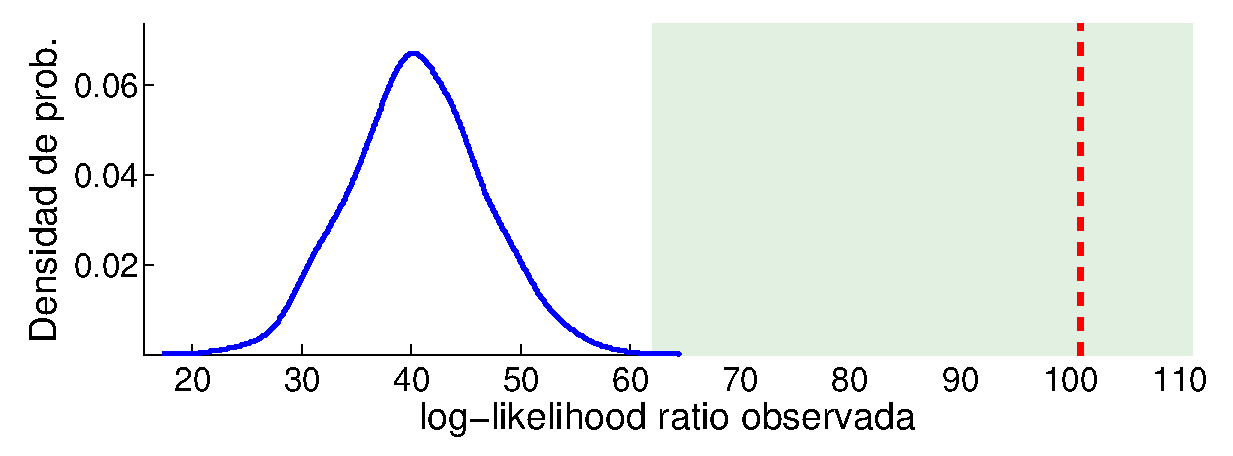
\includegraphics[width=1\linewidth]{gfx/chap6/calderon1boot1}
      \caption{}
      \label{fig:seq5_boot1}
    \end{subfigure}
    \hspace{0.5cm}
    \begin{subfigure}[b]{0.7\textwidth}
      \includegraphics[width=1\linewidth]{gfx/chap6/calderon1boot2}
      \caption{}
      \label{fig:seq5_boot2}
    \end{subfigure}
  }
  \centerline  
  { \begin{subfigure}[b]{0.7\textwidth}
      \includegraphics[width=1\linewidth]{gfx/chap6/calderon1boot3}
      \caption{}
      \label{fig:seq5_boot3}
    \end{subfigure}
    \hspace{0.5cm}
    \begin{subfigure}[b]{0.7\textwidth}
      \includegraphics[width=1\linewidth]{gfx/chap6/calderon1boot4}
      \caption{}
      \label{fig:seq5_boot4}
    \end{subfigure}
  }
  \caption[Secuencia 5: Pruebas de hipótesis usando bootstrap]{En la \autoref{fig:seq5_boot1} se muestra la prueba de hipótesis realizada para comparar el modelo $n_2$ contra $n_3$. Como se observa, se rechaza la hipótesis de que el modelo correcto sea $n_2$. En la \autoref{fig:seq5_boot2} se hace la prueba del modelo $n_3$ contra $n_4$, y se vuelve a rechazar la hipótesis nula, aunque queda muy cerca del umbral de decisión. Realizando la prueba de $n_4$ contra $n_5$ en la \autoref{fig:seq5_boot3} en este caso el valor observado no cae dentro de la región de rechazo, por lo que no podemos rechazar que el modelo $n_4$ sea el correcto. Por último en la \autoref{fig:seq5_boot4}, se hace la prueba del modelo $n_5$ contra el modelo $n_5$, y vuelve a suceder lo mismo que en el caso anterior. Como para las últimas dos pruebas no se pudo rechazar la hipótesis nula, se preferirá siempre la que involucre al modelo más sencillo. Cabe recalcar también que si se hicieran las pruebas de hipótesis con una significancia menor, entonces desde la segunda prueba se tendría al modelo ganador,}
  \label{fig:seq5_boot}
\end{figure}

En caso de que después de utilizar BIC se presente ambigüedad para determinar un modelo ganador, o ya sea para realizar un análisis más exhaustivo, se puede propone hacer una prueba de hipótesis para determinar cuál modelo se ajusta mejor a los datos.

A diferencia de la primer etapa, en la que se usa BIC como criterio para  seleccionar el mejor modelo de un conjunto no definido de modelos con diferentes parámetros, la intención de hacer pruebas de hipótesis es determinar en un pequeño conjunto de probables modelos, cuál es mejor, y qué tan bueno es un modelo respecto a otro.

Al plantear la prueba de hipótesis se harán una gran cantidad de simulaciones para ver qué tan bien se ajusta cada modelo a los datos originales, por lo que este proceso es computacionalmente intensivo y sólo se recomienda hacerlo para evitar la ambigüedad entre un par de modelos.

...

Por último, ya con el modelo seleccionado, se procede a calcular el error relativo de predicción que se obtuvo, comparando con el ground truth que se dispone para esa secuencia, con lo que se obtiene: 

...

\begin{figure}[bht]
  \centerline
  {\begin{subfigure}[b]{1.3\textwidth}
      \includegraphics[width=1\linewidth]{gfx/chap6/calderon1s_3_1}
      \caption{}
      \label{fig:seq5_seq1}
    \end{subfigure}
  } 
  \centerline
  {\begin{subfigure}[b]{1.3\textwidth}
      \includegraphics[width=1\linewidth]{gfx/chap6/calderon1s_4_2}
      \caption{}
      \label{fig:seq5_seq3}
    \end{subfigure}
  }    
  \centerline
  {\begin{subfigure}[b]{1.3\textwidth}
      \includegraphics[width=1\linewidth]{gfx/chap6/calderon1s_3_2}
      \caption{}
      \label{fig:seq5_seq2}
    \end{subfigure}
  }
  \caption[Secuencia 5: Secuencia recuperada]{En \autoref{fig:seq5_seq1} se muestra la secuencia original de la \autoref{ssub:calderon}. En comparación, en \autoref{fig:seq5_seq3} se muestra la secuencia recuperada del modelo ganador y se marcan en rojo los errores cometidos respecto a la primera secuencia. Por último, se muestra en \autoref{fig:seq5_seq2} la el modelo que debió haber ganado en caso de que se usara una significacia más baja para las pruebas.}
  \label{fig:prb5_seq}
\end{figure}

Más a detalle, en la \autoref{fig:prb5_seq} se observa en azul el orden en el que participan los interlocutores de acuerdo a la secuencia recuperada. En rojo se marcan tanto los falsos positivos como los falsos negativos, de acuerdo al ground truth. Hay que notar que cuando el número de estados para un modelo no es el correcto, entonces inminentemente el número de errores en la secuencia obtenida será mayor, pues al menos todas las intervenciones de un hablante no podrán ser emparejadas o serán asignadas a alguien más.

Se observa también que la mayoría de las veces, en la secuencia recuperada se encuentran algunos brincos entre personas, pero en esencia la estructura y el orden en que hablan los interlocutores es el correcto.
 
  
%%%%%%%%%%%%%%%%%%%%%%%%%%%%%%%%%%%%%%%%%%%%%%%%%%%%%%%%%%%%%%% 

\subsection[Secuencia 6]{Secuencia 6: Andrew Lloyd Webber}
\label{ssub:cats}

  Para la última secuencia de prueba se utilizaron fragmentos de la obra musical 'Cats', escrita por Andrew Lloyd Webber, usando 5 voces distintas en inglés. La secuencia de audio original tiene una duración de 6:48 min.

Para la etapa de agrupación de los vectores MFCC con k-means++ se usaron 90 centros iniciales, usando el mismo banco de filtros.

\begin{figure}[tp]
  \centerline{  
    \hspace{1.2cm}
    \parbox[c]{0.38\textwidth}{\centering Modelo generador}
    \parbox[c]{0.38\textwidth}{\centering Modelo $n_4$}
    \parbox[c]{0.38\textwidth}{\centering Modelo $n_5$}
    \parbox[c]{0.38\textwidth}{\centering Modelo $n_6$}
  }
  \vspace{0.5cm}
  \foreach \row in {1, ..., 2}{%  
    \centerline{%
      \parbox[c]{1cm}{
        \vspace{-0.5cm}
        \myheader{\row}
      }
      %\gdef \widthimg {0.35}
      \foreach \col in {1, ..., 4}{%
        \pgfmathparse{\col == 4 && \row == 2? 1:0}
        \ifthenelse{\pgfmathresult=1}{
          \gdef \widthimg {0.39}
        }{
          \gdef \widthimg {0.35}
        }
        \begin{subfigure}[c]{\widthimg \textwidth}          
          \def \imgfile {gfx/chap6/cats1p_\col_\row}
          \IfFileExists{\imgfile.eps}{
            \includegraphics[width=1\textwidth]{\imgfile}
            \label{fig:seq6p_\col_\row}
          }{
            \hspace{1\textwidth}
          }
        \end{subfigure}
        %\hspace{-0.005\textwidth}
      }
    }
  }
\caption[Secuencia 6: Parámetros estimados (1)]{Por columnas, se muestran los parámetros obtenidos para varios modelos propuestos. La primer columna corresponde a los parámetros verdaderos.
En la primer fila \textup{(a)} se muestran las probabilidades a priori de que cada uno de los interlocutores empiecen la conversación. En la segunda fila \textup{(b)} se muestra en falso color la matriz de transición entre interlocutores para cada uno de los modelos mostrados.}
\label{fig:seq6p}
\end{figure}

En las \autoref{fig:seq6p} y \autoref{fig:seq6q} se muestran los parámetros estimados para los diferentes modelos que se propusieron. La primer columna corresponde a los parámetros verdaderos, mientras que las demás columnas son los parámetros obtenidos para diferentes modelos estimados. 

En la primer fila de la \autoref{fig:seq6p} se muestran las probabilidades a priori de que cada uno de los interlocutores empiecen el diálogo. En la segunda fila se muestra en falso color la matriz de transición para cada uno de los modelos. Esta matriz representa la probabilidad de cambio entre las personas que participan en la conversación.

Se observa como en general para todos los modelos propuestos la matriz de transición que se recupera tiene una estructura diagonal, puesto que en este tipo de problemas, una persona suele hablar durante un periodo considerablemente largo, para que luego otra persona empiece a hablar.

\begin{figure}[t!]
  \centerline{
    \hspace{1.2cm}
    \parbox[c]{0.35\textwidth}{\centering Modelo generador}
    \parbox[c]{0.35\textwidth}{\centering Modelo $n_4$}
    \parbox[c]{0.35\textwidth}{\centering Modelo $n_5$}
    \parbox[c]{0.35\textwidth}{\centering Modelo $n_6$}
  }
  \vspace{0.5cm}
  \foreach \row in {3, ..., 8}{%  
    \centerline{
      \parbox[c]{1cm}{
        \vspace{-0.3cm}
        \myheader{\row}
      }
      \foreach \col in {1, ..., 4}{%
        \begin{subfigure}[c]{0.35\textwidth}  
          \def \imgfile {gfx/chap6/cats1p_\col_\row}
          \IfFileExists{\imgfile.eps}{
            \includegraphics[width=1\textwidth]{\imgfile}
            %\caption{}
            \label{fig:seq6p_\col_\row}
          }{
            \hspace{1\textwidth}
          }
        \end{subfigure}
      }
    }
  }
\caption[Secuencia 6: Parámetros estimados (2)]{Por columnas, se muestran las probabilidades de emisión para cada uno de los interlocutores de acuerdo al modelo. Cada fila representa las probabilidad de emisión de las palabras en el diccionario. La fila \textup{(c)} para la primer persona, la fila \textup{(d)} para la segunda persona y así de forma consecutiva, de acuerdo al número de personas que contempla cada modelo propuesto.}
\label{fig:seq6q}
\end{figure}

En la \autoref{fig:seq6q} se muestran las probabilidades de emisión para cada uno de los participantes, de acuerdo a las palabras en las que se ha discretizado la conversación. Idealmente, cada interlocutor tiene asignadas con mayor probabilidad un cierto conjunto de palabras del diccionario, lo que hace que la identificación de las personas sea mucho más fácil de realizar.

Para la selección del modelo y siguiendo la metodología propuesta, primero se efectúa una inspección por medio de BIC regularizado para encontrar cuál o cuáles son los modelos más probables.

\begin{figure}[t!]
  \centerline{
  \begin{subfigure}[b]{1.1\textwidth}
   \includegraphics[width=1\textwidth]{gfx/chap6/noct1bic2}
   \caption{}
   \label{fig:seq6_bic2}
  \end{subfigure}  
  }  
  \centerline{
  \begin{subfigure}[b]{0.55\textwidth}
    \includegraphics[width=\textwidth]{gfx/chap6/noct1bic1} 
    \caption{}
    \label{fig:seq6_bic1}
  \end{subfigure}  
  \begin{subfigure}[b]{0.55\textwidth}
    \includegraphics[width=\textwidth]{gfx/chap6/lear3bic3} 
    \caption{}
    \label{fig:seq6_bic3}
  \end{subfigure}
  }
  \caption[Secuencia 6: Pruebas BIC]{En la \autoref{fig:seq6_bic2}, se muestra las curvas de nivel de la superficie al variar el valor de lambda para evaluar BIC, así como la dirección del gradiente en la misma. En la \autoref{fig:seq6_bic1} se muestra una perspectiva general de superficie en \autoref{fig:seq6_bic2}. En la \autoref{fig:seq6_bic3} se muestra el valor seleccionado para lambda de acuerdo al análisis de sensibilidad realizado en la superficie anterior.}
  \label{fig:seq6_bic}
\end{figure}

En la \autoref{fig:seq6_bic1} se muestra la superficie generada al variar el valor de $\lambda$ para diferentes curvas de selección BIC. Se observa cómo al principio $\lambda$ es muy pequeño, y entonces el término de penalización no funciona por lo que se prefieren los modelos más complejos y sobre ajustados. Por otro lado, cuando $\lambda$ es muy grande, la penalización no permite mas que escoger los modelos más simples.

Haciendo un análisis de sensibilidad se puede determinar cuál es el parámetro $\lambda$ adecuado que penaliza de buena forma la log-verosimilitud.

En la \autoref{fig:seq6_bic2} se muestran las curvas de nivel de la figura anterior, además de la dirección del gradiente de la misma. Así mismo, en falso color se resaltan las zonas en las que el gradiente es menor. 

Lo que nos interesa encontrar en la superficie, es el valor de $\lambda$ que representa el punto de inflexión entre la selección de modelos demasiado complejos y modelos más simples. Para esto, se busca la zona en la que el gradiente sea lo más cercano a cero, pues implicaría que es un punto crítico.

Debido a la escala y a la forma en la que se calculó el gradiente, aunque para algunos valores cercanos de $\lambda$ no haya mucha variación en esa dirección; si BIC está penalizando mal, entonces sí habrá gran variación para los diferentes modelos. Es por esto, que sólo en la zona en que la penalización sea del mismo orden de magnitud que la verosimilitud la variación en la curva BIC con el $\lambda$ adecuado no será tan grande como en otras zonas.

Por último, se muestra en \autoref{fig:seq6_bic3} la curva BIC con el valor de $\lambda$ encontrado a partir del análisis de sensibilidad realizado en la \autoref{fig:seq6_bic2}. El o los modelos que tengan un mayor valor BIC serán los que se seleccionarán como modelos ganadores.

\begin{figure}[t!]
  \centerline  
  { \begin{subfigure}[b]{0.7\textwidth}
      \includegraphics[width=1\linewidth]{gfx/chap6/cats1boot1}
      \caption{}
      \label{fig:seq6_boot1}
    \end{subfigure}
    \hspace{0.5cm}
    \begin{subfigure}[b]{0.7\textwidth}
      \includegraphics[width=1\linewidth]{gfx/chap6/cats1boot2}
      \caption{}
      \label{fig:seq6_boot2}
    \end{subfigure}
  }
  \centerline  
  { \begin{subfigure}[b]{0.7\textwidth}
      \includegraphics[width=1\linewidth]{gfx/chap6/cats1boot3}
      \caption{}
      \label{fig:seq6_boot3}
    \end{subfigure}
    \hspace{0.5cm}
    \begin{subfigure}[b]{0.7\textwidth}
      \includegraphics[width=1\linewidth]{gfx/chap6/cats1boot4}
      \caption{}
      \label{fig:seq6_boot4}
    \end{subfigure}
  }
  \caption[Secuencia 6: Pruebas de hipótesis usando bootstrap]{En la \autoref{fig:seq6_boot1} se muestra la prueba de hipótesis realizada para comparar el modelo $n_4$ contra $n_5$. Como se observa, se rechaza la hipótesis de que el modelo correcto sea $n_4$. En la \autoref{fig:seq6_boot2} se hace la prueba del modelo $n_5$ contra $n_6$, y de la misma manera, se rechaza la hipótesis de que el modelo correcto sea $n_5$. Se sigue con la prueba de hipótesis del modelo $n_6$ contra $n_7$ en la \autoref{fig:seq6_boot3}, y en este caso el valor observado no cae dentro de la región de rechazo, por lo que no podemos rechazar que el modelo $n_6$ sea el correcto. Por último en la \autoref{fig:seq6_boot4}, se hace la prueba del modelo $n_7$ contra el modelo $n_8$, y se vuelve a rechazar la hipótesis nula.}  
  \label{fig:seq4_boot}
\end{figure}

En caso de que después de utilizar BIC se presente ambigüedad para determinar un modelo ganador, o ya sea para realizar un análisis más exhaustivo, se puede propone hacer una prueba de hipótesis para determinar cuál modelo se ajusta mejor a los datos.

A diferencia de la primer etapa, en la que se usa BIC como criterio para  seleccionar el mejor modelo de un conjunto no definido de modelos con diferentes parámetros, la intención de hacer pruebas de hipótesis es determinar en un pequeño conjunto de probables modelos, cuál es mejor, y qué tan bueno es un modelo respecto a otro.

Al plantear la prueba de hipótesis se harán una gran cantidad de simulaciones para ver qué tan bien se ajusta cada modelo a los datos originales, por lo que este proceso es computacionalmente intensivo y sólo se recomienda hacerlo para evitar la ambigüedad entre un par de modelos.

...

Por último, ya con el modelo seleccionado, se procede a calcular el error relativo de predicción que se obtuvo, comparando con el ground truth que se dispone para esa secuencia, con lo que se obtiene: 

...

\begin{figure}[tp]
  \centerline
  {\begin{subfigure}[b]{1.3\textwidth}
      \includegraphics[width=1\linewidth]{gfx/chap6/cats1s_3_1}
      \caption{}
      \label{fig:seq6_seq1}
    \end{subfigure}
  } 
  \centerline
  {\begin{subfigure}[b]{1.3\textwidth}
      \includegraphics[width=1\linewidth]{gfx/chap6/cats1s_3_2}
      \caption{}
      \label{fig:seq6_seq2}
    \end{subfigure}
  }
  \caption[Secuencia 6: Secuencia recuperada]{En \autoref{fig:seq6_seq1} se muestra la secuencia original de la \autoref{ssub:cats}. En comparación, en \autoref{fig:seq6_seq2} se muestra la secuencia recuperada del modelo ganador y se marcan en rojo los errores cometidos respecto a la primera secuencia. }
  \label{fig:prb6_seq}
\end{figure}

Más a detalle, en la \autoref{fig:prb6_seq} se observa en azul el orden en el que participan los interlocutores de acuerdo a la secuencia recuperada. En rojo se marcan tanto los falsos positivos como los falsos negativos, de acuerdo al ground truth. Hay que notar que cuando el número de estados para un modelo no es el correcto, entonces inminentemente el número de errores en la secuencia obtenida será mayor, pues al menos todas las intervenciones de un hablante no podrán ser emparejadas o serán asignadas a alguien más.

Se observa también que la mayoría de las veces, en la secuencia recuperada se encuentran algunos brincos entre personas, pero en esencia la estructura y el orden en que hablan los interlocutores es el correcto.
   


\section{Resultados}

A continuación se presentan la tabla \autoref{tab:example} los resultados condensados de las pruebas realizadas con las secuencias antes descritas.

\begin{table}
  \centerline {
  \begin{tabularx}{1.2\textwidth}{X rrrccc} \toprule
    \tableheadline{Sec. Id.}& 
  	\tableheadline{Duración} & 
  	\tableheadline{$\#_{SAMPLES}$} &
  	\tableheadline{$\#_{WORDS}$} &  	
  	\tableheadline{$n_{TRUE}$} &
  	\tableheadline{$n_{FOUND}$} & 
    \tableheadline{DER} 	
	  \\ \midrule
    ALLPOE~ & 12:06 min & 7218 & 140 & 6 & 6 & 0.03324 \\ 
    GARMÁR~ &  6:55 min & 4154 &  90 & 4 & 4 & 0.00652 \\
    WSHAKE~ &  2:43 min & 1636 & 160 & 4 & 4 & 0.03324 \\ 
    MACUÑA~ & 10:41 min & 6414 & 120 & 3 & 3 & 0.00343 \\ 
    CALDER~ &  1:07 min &  676 & 160 & 3 & 3 & 0.08092 \\ 
    LLOYDW~ &  6.48 min & 4084 & 160 & 5 & 5 & 0.01170 \\    
    \bottomrule
  \end{tabularx} 
  }
  \caption[as]{asdasd}  
  \label{tab:example}
\end{table}
